% ============================================================================
% PONTIFICIA UNIVERSIDAD JAVERIANA
% FACULTAD DE INGENIERIA - SISTEMAS
% Observatorio de Demanda Laboral en América Latina
% ============================================================================

\documentclass[11pt,oneside,letterpaper]{report}

% ============================================================================
% PAQUETES
% ============================================================================
\usepackage[utf8]{inputenc}
\usepackage[spanish,es-tabla]{babel}
\usepackage[letterpaper,top=3cm,bottom=3cm,left=3cm,right=3cm]{geometry}
\usepackage{times}
\usepackage{graphicx}
\usepackage{amsmath,amssymb}
\usepackage{setspace}
\usepackage{fancyhdr}
\usepackage{titlesec}
\usepackage{tocloft}
\usepackage[hidelinks]{hyperref}
\usepackage{listings}
\usepackage{xcolor}
\usepackage{float}
\usepackage{longtable}
\usepackage{multirow}
\usepackage{array}
\usepackage[backend=biber,style=ieee,citestyle=numeric-comp,sorting=none]{biblatex}

% TikZ para diagramas
\usepackage{tikz}
\usetikzlibrary{shapes.geometric, arrows.meta, positioning, shadows, fit, shapes.multipart}

% ============================================================================
% CONFIGURACIÓN DE BIBLIOGRAFÍA
% ============================================================================
\addbibresource{bibliografia.bib}

% ============================================================================
% CONFIGURACIÓN DE CÓDIGO
% ============================================================================
\lstset{
    basicstyle=\ttfamily\small,
    breaklines=true,
    frame=single,
    numbers=left,
    numberstyle=\tiny\color{gray},
    keywordstyle=\color{blue},
    commentstyle=\color{green!60!black},
    stringstyle=\color{orange},
    showstringspaces=false
}

% ============================================================================
% CONFIGURACIÓN DE INTERLINEADO
% ============================================================================
\onehalfspacing

% ============================================================================
% CONFIGURACIÓN DE ENCABEZADOS Y PIE DE PÁGINA
% ============================================================================
\pagestyle{fancy}
\fancyhf{}
\fancyhead[L]{Pontificia Universidad Javeriana}
\fancyhead[R]{Informe de Proyecto de Grado}
\fancyfoot[R]{Página \thepage}
\renewcommand{\headrulewidth}{0.4pt}
\renewcommand{\footrulewidth}{0.4pt}

% Forzar que la primera página de cada capítulo use el mismo estilo
\fancypagestyle{plain}{%
  \fancyhf{}%
  \fancyhead[L]{Pontificia Universidad Javeriana}
  \fancyhead[R]{Informe de Proyecto de Grado}
  \fancyfoot[R]{Página \thepage}
  \renewcommand{\headrulewidth}{0.4pt}
  \renewcommand{\footrulewidth}{0.4pt}
}

% ============================================================================
% CONFIGURACIÓN DE TÍTULOS DE CAPÍTULOS
% ============================================================================
\titleformat{\chapter}[display]
{\normalfont\Large\bfseries\centering}
{}{0pt}{\Large}

\titlespacing*{\chapter}{0pt}{20pt}{20pt}

\titleformat{\section}
{\normalfont\large\bfseries}{\thesection}{1em}{}

\titleformat{\subsection}
{\normalfont\normalsize\bfseries}{\thesubsection}{1em}{}

% ============================================================================
% INFORMACIÓN DEL PROYECTO
% ============================================================================
\newcommand{\proyectoTitulo}{Observatorio de demanda laboral en América Latina}
\newcommand{\proyectoCodigo}{CIS2025CP08}
\newcommand{\autorUno}{Nicolas Francisco Camacho Alarcón}
\newcommand{\autorDos}{Alejandro Pinzón Fajardo}
\newcommand{\director}{Ing. Luis Gabriel Moreno Sandoval}
\newcommand{\juradoUno}{Ing. <<Nombre Jurado 1>>}
\newcommand{\juradoDos}{Ing. <<Nombre Jurado 2>>}
\newcommand{\anio}{2025}
\newcommand{\mes}{Noviembre}

% ============================================================================
% DOCUMENTO
% ============================================================================
\begin{document}

% Páginas preliminares con numeración romana
\pagenumbering{roman}

% Portada principal
\begin{titlepage}
    \centering

    % Grupo en la parte superior
    \vspace*{1cm}
    {\large\bfseries Grupo 8\par}

    \vspace{4cm}

    % Título del proyecto
    {\LARGE\bfseries \proyectoTitulo\par}

    \vspace{4cm}

    % Autores
    {\large \autorUno\par}
    \vspace{0.3cm}
    {\large \autorDos\par}

    \vfill

    % Información de la universidad
    {\large PONTIFICIA UNIVERSIDAD JAVERIANA\par}
    {\large FACULTAD DE INGENIERÍA\par}
    {\large CARRERA DE INGENIERÍA DE SISTEMAS\par}
    {\large BOGOTÁ, D.C.\par}
    {\large \anio\par}

\end{titlepage}

\newpage

% Página en blanco
\thispagestyle{empty}
\mbox{}
\newpage

% Portada interna
\thispagestyle{fancy}

\begin{center}
    {\large\bfseries \proyectoCodigo\par}
    \vspace{0.5cm}
    {\large\bfseries \proyectoTitulo\par}
\end{center}

\vspace{3cm}

\begin{center}
    {\large\bfseries Author(s):\par}
    \vspace{0.5cm}
    {\large \autorUno\par}
    {\large \autorDos\par}
\end{center}

\vspace{3cm}

\begin{center}
    UNDERGRADUATE FINAL PROJECT REPORT PERFORMED IN ORDER TO ACCOMPLISH ONE OF THE REQUIREMENTS FOR THE SYSTEMS ENGINEERING DEGREE
\end{center}

\vspace{2cm}

\begin{center}
    {\large\bfseries Director\par}
    \vspace{0.5cm}
    {\large \director\par}

    \vspace{1.5cm}

    {\large\bfseries Juries of the Undergraduate Final Project\par}
    \vspace{0.5cm}
    {\large \juradoUno\par}
    {\large \juradoDos\par}
\end{center}

\vfill

\begin{center}
    {\large PONTIFICIA UNIVERSIDAD JAVERIANA\par}
    {\large FACULTAD DE INGENIERIA\par}
    {\large SYSTEMS ENGINEERING PROGRAM\par}
    {\large BOGOTÁ, D.C.\par}
    {\large \mes, \anio\par}
\end{center}

\newpage

% Autoridades
\thispagestyle{fancy}
\fancyfoot[R]{Page iii}

\begin{center}
    {\large\bfseries PONTIFICIA UNIVERSIDAD JAVERIANA\par}
    {\large\bfseries FACULTAD DE INGENIERIA\par}
    {\large\bfseries SYSTEMS ENGINEERING PROGRAM\par}
\end{center}

\vspace{4cm}

\begin{center}
    {\large\bfseries President of the Pontificia Universidad Javeriana\par}
    \vspace{0.5cm}
    {\large <Name of the President of the University>\par}

    \vspace{2cm}

    {\large\bfseries Dean of School of Engineering\par}
    \vspace{0.5cm}
    {\large <Name of the Dean>\par}

    \vspace{2cm}

    {\large\bfseries Head of the Systems Engineering Program\par}
    \vspace{0.5cm}
    {\large <Name of the head of the program>\par}

    \vspace{2cm}

    {\large\bfseries Head of the Systems Engineering Department\par}
    \vspace{0.5cm}
    {\large <Name of the head of the department>\par}
\end{center}

\newpage

% Artículo 23
\thispagestyle{fancy}
\fancyfoot[R]{Page iv}

{\large\bfseries Artículo 23 de la Resolución No. 1 de Junio de 1946}

\vspace{1cm}

\textit{``La Universidad no se hace responsable de los conceptos emitidos por sus alumnos en sus proyectos de grado. Sólo velará porque no se publique nada contrario al dogma y la moral católica y porque no contengan ataques o polémicas puramente personales. Antes bien, que se vean en ellos el anhelo de buscar la verdad y la Justicia''}

\newpage

% Agradecimientos
\thispagestyle{fancy}

\begin{center}
    {\large\bfseries GRATITUDE}
\end{center}

\vspace{1cm}

\textit{Write a message if you feel gratitude for someone who has supported the development of the project. Your family, your partner, your friends, your principal, teachers, etc.}

\newpage

% Tabla de contenidos
\renewcommand{\contentsname}{CONTENIDO}
\tableofcontents
\newpage

% Abstract
\thispagestyle{fancy}
\fancyfoot[R]{Page vii}

\begin{center}
    {\large\bfseries ABSTRACT}
\end{center}

\vspace{1cm}

El desajuste entre las habilidades demandadas por el mercado y la oferta formativa en Latinoamérica dificultaba decisiones de política, academia y empresa. Este proyecto abordó el problema construyendo un observatorio automatizado que recolectó avisos de empleo multi-portal y multi-país, escalable hacia $\sim$600.000 registros. Se integraron spiders (Scrapy/Selenium con anti-detección), una base PostgreSQL con pgvector y un pipeline de extracción/normalización de habilidades (NER/regex con apoyo LLM) alineadas a ESCO. El sistema generó indicadores, consultas y visualizaciones reproducibles, entregando evidencia comparable por país, sector y tiempo para orientar currículos, formación y estrategias de talento.


% ============================================================================
% CAPÍTULOS PRINCIPALES - Numeración arábiga desde página 1
% ============================================================================
\clearpage
\pagestyle{fancy}
\pagenumbering{arabic}

\chapter{INTRODUCCIÓN}

Los mercados laborales latinoamericanos evolucionan con rapidez y publican sus vacantes en portales heterogéneos, con formatos dispares, vocabularios no estandarizados y alta volatilidad (los avisos desaparecen o cambian con frecuencia). Esta fragmentación dificulta medir, con evidencia objetiva y comparable, qué habilidades técnicas y digitales están siendo demandadas por país, sector y momento del tiempo. El proyecto \textbf{Observatorio de Demanda Laboral para América Latina} responde a ese vacío mediante un sistema automatizado que captura, estructura y analiza anuncios de empleo a escala.

La solución integra un \textbf{pipeline} modular de ocho etapas: Scraping multifuente y multipaís (Colombia, México, Argentina) con spiders robustos y medidas anti-detección; Normalización y limpieza; Extracción de habilidades combinando NER, patrones regex y apoyo LLM; Alineación a la taxonomía ESCO; Generación de embeddings multilingües (modelo E5); Reducción dimensional (UMAP); Clustering (HDBSCAN) para descubrir familias de perfiles; y Visualización y reportes. La infraestructura técnica se apoya en \textbf{Python/Scrapy, PostgreSQL + pgvector} y \textbf{Docker}, con registro y monitorización de extremo a extremo.

Este documento guía al lector desde el contexto y la motivación hasta los resultados y conclusiones. Presenta: I) antecedentes y trabajos relacionados; II) arquitectura del sistema y orquestación; III) adquisición y modelado de datos; IV) métodos de extracción y normalización de habilidades; V) componentes de representación y análisis; VI) evaluación y métricas; VII) hallazgos y visualizaciones; VIII) consideraciones éticas y limitaciones; y IX) conclusiones y trabajo futuro.

\chapter{DESCRIPCIÓN GENERAL}

\section{Oportunidad y problema}

\subsection{Contexto del problema}

El mercado laboral en América Latina se encontró, durante la última década, en una compleja encrucijada definida por la confluencia de dos fuerzas a menudo contrapuestas: una acelerada transformación digital y la persistencia de desafíos estructurales, como una elevada informalidad laboral y brechas de capital humano \cite{echeverria2022}. La pandemia de COVID-19 actuó como un catalizador sin precedentes, intensificando la adopción de tecnologías y, con ello, la demanda de competencias digitales, al tiempo que exponía la vulnerabilidad de los mercados de trabajo de la región \cite{azuara2022}. Este dinamismo generó el riesgo de que la automatización y la digitalización, de no ser gestionadas estratégicamente, pudiesen exacerbar las desigualdades existentes, conduciendo a una mayor polarización y segmentación social \cite{echeverria2022}.

Para analizar este fenómeno regional de manera tangible y robusta, este proyecto seleccionó como casos de estudio a tres de las economías más grandes y digitalmente activas de habla hispana: Colombia, México y Argentina. La elección de estos países respondió a tres criterios estratégicos. Primero, su alto volumen de publicaciones de ofertas laborales en portales digitales aseguró la viabilidad de una recolección masiva de datos (web scraping), fundamental para el entrenamiento de modelos de lenguaje robustos \cite{aguilera2018, martinez2024, rubio2025}. Segundo, la existencia de estudios previos en cada país, aunque metodológicamente limitados, confirmó la pertinencia del problema y proporcionó una línea de base para la comparación \cite{cardenas2015, campos2024}. Y tercero, su diversidad en términos de realidades económicas, territoriales y de madurez digital permitió validar que la solución desarrollada fuese portable y adaptable a los distintos contextos que caracterizan a América Latina.

El caso de Colombia sirvió como una ilustración profunda de esta dinámica. El diagnóstico nacional previo al proyecto ya indicaba que el principal cuello de botella para la inclusión digital no era la falta de infraestructura, sino la brecha de capital humano. Específicamente, el ``Índice de Brecha Digital'' (IBD) del Ministerio de Tecnologías de la Información y las Comunicaciones reveló que la dimensión de ``Habilidades Digitales'' constituía el mayor componente individual de la brecha en el país. Esta evidencia fue posteriormente corroborada y cuantificada por el análisis empírico de la demanda laboral, el cual demostró que la pandemia generó un cambio estructural y persistente en el mercado. Se encontró que, en los 18 meses posteriores al inicio de la crisis sanitaria, las vacantes tecnológicas aumentaron en un 50\% en comparación con las no tecnológicas \cite{rubio2025}. Este cambio no fue solo cuantitativo, sino también cualitativo: se observó una marcada caída en la demanda de herramientas ofimáticas tradicionales como Excel (cuya mención en ofertas cayó del 35.8\% en 2018 al 17.4\% en 2023) y un surgimiento exponencial de tecnologías especializadas asociadas al desarrollo web y la gestión de datos, como bases de datos NoSQL (12.3\%), el framework Django (5.5\%) y la librería React (5.3\%) para el año 2023 \cite{rubio2025}.

\subsection{Formulación del problema}

A pesar de que el contexto del problema ---la creciente e insatisfecha demanda de habilidades tecnológicas--- estaba claramente identificado, los métodos existentes en la región para analizarlo presentaban limitaciones metodológicas significativas que impedían una comprensión profunda y ágil del fenómeno. Los estudios de referencia en los países seleccionados, si bien valiosos para establecer tendencias macro, se basaron en enfoques de análisis léxico y reglas manuales. En Colombia, el análisis se centró en un sistema de clasificación basado en la Clasificación Internacional Uniforme de Ocupaciones (CIUO), utilizando algoritmos de emparejamiento de texto con tokenización y métricas de similitud basadas en n-gramas \cite{rubio2025}. De forma análoga, en Argentina, los estudios se concentraron en técnicas de minería de texto con análisis de frecuencias y bigramas para identificar patrones en las ofertas del sector TI \cite{aguilera2018}. En México, el enfoque combinó datos de encuestas con scraping de portales, apoyándose en el análisis de frecuencia de términos y la creación de tipologías manuales para segmentar las habilidades \cite{martinez2024}.

La limitación fundamental compartida por estos enfoques es su dependencia de la correspondencia léxica explícita, lo que los hace incapaces de capturar la riqueza semántica del lenguaje. Estos métodos no podían detectar habilidades implícitas (aquellas que se infieren del contexto de un cargo pero no se mencionan directamente), gestionar la ambigüedad del lenguaje informal o el uso de anglicismos técnicos (``Spanglish''), ni identificar clústeres de competencias emergentes que aún no forman parte de taxonomías estandarizadas. La alta variabilidad en la redacción de las ofertas laborales, la falta de estructuras normalizadas y la rápida aparición de nuevas tecnologías hacían que estos sistemas fueran metodológicamente frágiles y requirieran un constante mantenimiento manual \cite{echeverria2022, lukauskas2023}.

En consecuencia, el problema específico que este proyecto abordó fue la ausencia de una herramienta automatizada y de extremo a extremo que, adaptada a las particularidades lingüísticas y estructurales del español latinoamericano, permitiera superar las limitaciones de los análisis léxicos tradicionales. Se identificó la necesidad de un sistema capaz de extraer, estructurar y analizar la evolución de las habilidades tecnológicas de manera semántica, escalable y con un mayor grado de autonomía, integrando para ello técnicas avanzadas de Procesamiento de Lenguaje Natural (NLP), enriquecimiento contextual con Large Language Models (LLMs) y algoritmos de agrupamiento no supervisado.

\subsection{Propuesta de solución}

Para dar respuesta al problema formulado, se diseñó e implementó un observatorio de demanda laboral tecnológica basado en un pipeline modular y automatizado, un proyecto enmarcado en las áreas de Ingeniería de Sistemas y Ciencia de Datos. El sistema fue concebido como una solución de extremo a extremo que integró las etapas de recolección, procesamiento, análisis semántico y segmentación de ofertas de empleo publicadas en Colombia, México y Argentina. El objetivo fue crear una arquitectura robusta, replicable y adaptada a las complejidades del contexto latinoamericano, superando las limitaciones de los enfoques puramente léxicos o manuales.

La solución se materializó a través de un sistema compuesto por módulos secuenciales y cohesivos. El primer módulo consistió en un motor de adquisición de datos que, mediante técnicas de web scraping, extrajo de forma sistemática y ética decenas de miles de ofertas laborales de portales de empleo clave en la región. El núcleo del sistema fue su arquitectura de extracción dual, compuesta por dos pipelines paralelos:

\textbf{Pipeline A (Tradicional):} Implementó un método de extracción basado en Reconocimiento de Entidades Nombradas (NER) utilizando un EntityRuler de spaCy, poblado con la taxonomía completa de ESCO, combinado con expresiones regulares para capturar un baseline de habilidades explícitas de alta precisión.

\textbf{Pipeline B (Basado en LLMs):} Empleó Large Language Models (LLMs) como Llama 3 para realizar una extracción semántica, capaz de identificar no solo habilidades explícitas sino también de inferir competencias implícitas a partir del contexto de la vacante, siguiendo enfoques de vanguardia \cite{herandi2024, nguyen2024}.

Posteriormente, un módulo de mapeo de dos capas normalizó las habilidades extraídas por ambos pipelines contra la taxonomía ESCO. La primera capa realizó una coincidencia léxica (exacta y difusa), mientras que la segunda ejecutó una búsqueda de similitud semántica de alto rendimiento, utilizando embeddings multilingües (E5) y un índice FAISS pre-calculado, inspirado en las arquitecturas de herramientas como ESCOX \cite{kavargyris2025}. Finalmente, un módulo de análisis no supervisado aplicó una secuencia metodológica de embeddings, reducción de dimensionalidad con UMAP y agrupamiento con HDBSCAN para identificar clústeres de habilidades y perfiles emergentes, un enfoque validado por la literatura para el descubrimiento de estructuras en el mercado laboral \cite{lukauskas2023}.

\subsection{Justificación de la solución}

La solución implementada se justificó como una alternativa superior y mejor adaptada para el análisis de la demanda de habilidades en América Latina, ya que abordó directamente las debilidades metodológicas identificadas en los estudios previos. A diferencia de los enfoques basados exclusivamente en reglas léxicas \cite{aguilera2018, rubio2025} o en el uso aislado de LLMs \cite{nguyen2024}, la arquitectura de dos pipelines paralelos permitió una validación empírica cruzada: combinó la auditabilidad y alta precisión para habilidades conocidas del Pipeline A con la potencia inferencial y la capacidad de descubrir habilidades implícitas del Pipeline B. Este diseño comparativo proveyó un marco para evaluar objetivamente el rendimiento de los LLMs, en lugar de depender únicamente de su capacidad ``black-box''.

Técnicamente, el sistema representó un avance significativo en escalabilidad y eficiencia. La implementación de un índice FAISS para la búsqueda semántica de similitud (una mejora sobre la propuesta original de ESCOX) permitió procesar grandes volúmenes de datos a una velocidad órdenes de magnitud superior a las búsquedas en bases de datos vectoriales convencionales, haciendo factible el análisis de todo el corpus recolectado \cite{kavargyris2025, lukauskas2023}. Adicionalmente, el sistema fue diseñado explícitamente para la realidad del español latinoamericano. Este enfoque abordó directamente una limitación crítica de trabajos de vanguardia en LLMs, los cuales se han desarrollado y validado casi exclusivamente sobre datasets en inglés \cite{herandi2024}, ignorando las particularidades lingüísticas (como el ``Spanglish'') del dominio tecnológico en la región.

Finalmente, el valor agregado del proyecto residió en su síntesis estratégica de metodologías de vanguardia. El sistema no se limitó a una sola técnica, sino que articuló la cobertura del scraping regional, la potencia de los LLMs ajustados para generar salidas estructuradas \cite{herandi2024}, y la capacidad estructuradora del clustering semántico \cite{lukauskas2023}. Al hacerlo, se desarrolló un observatorio más completo, robusto y metodológicamente transparente que las alternativas existentes, estableciendo una base sólida y replicable para el monitoreo dinámico de la demanda laboral en la región.

\section{Descripción del proyecto}

El proyecto se concibió como un observatorio automatizado para capturar, normalizar y analizar avisos de empleo en Latinoamérica. Se integraron múltiples portales (CO, MX y AR), se diseñó una base de datos relacional con soporte vectorial, y se implementó un pipeline de extracción de habilidades (NER/regex/LLM) alineadas a ESCO, con generación de indicadores, visualizaciones y reportes. Operativamente, se planificó escalar hasta 600.000 avisos para la defensa, garantizando calidad, trazabilidad y reproducibilidad.

\subsection{Objetivo general}

Desarrollar un sistema que permita procesar y segmentar la demanda de habilidades tecnológicas en Colombia, México y Argentina, mediante técnicas de procesamiento de lenguaje natural.

\subsection{Objetivos específicos}

\begin{itemize}
    \item Construir un estado del arte exhaustivo para comparar trabajos existentes en el ámbito de observatorios laborales automatizados y técnicas de procesamiento de lenguaje natural en español.

    \item Diseñar una arquitectura modular, escalable y reutilizable para el observatorio laboral automatizado, fundamentada en las mejores prácticas identificadas en el estado del arte.

    \item Implementar e integrar técnicas de inteligencia artificial para la identificación, normalización y agrupación semántica de habilidades tecnológicas en ofertas laborales en español.

    \item Validar el desempeño y la robustez de la arquitectura y los modelos propuestos mediante métricas cuantitativas y estudios empíricos.
\end{itemize}

\subsection{Entregables, estándares y justificación}

\begin{longtable}{|p{5cm}|p{5cm}|p{5cm}|}
\hline
\textbf{Entregable} & \textbf{Estándares asociados} & \textbf{Justificación} \\
\hline
\endfirsthead

\hline
\textbf{Entregable} & \textbf{Estándares asociados} & \textbf{Justificación} \\
\hline
\endhead

\hline
\endfoot

\hline
\endlastfoot

Repositorio de código (spiders, orquestador, pipelines) & PEP 8/257/484; Conv. Commits; SemVer & Mantenibilidad, legibilidad y control de versiones. \\
\hline

Esquema BD y migraciones (PostgreSQL + pgvector) & Normalización (3NF); SQL best practices & Integridad, trazabilidad y soporte a consultas vectoriales. \\
\hline

Spiders y configuración de scraping & Polite crawling (delays/retries); manejo anti-bots & Captura estable a escala y resiliencia ante cambios UI. \\
\hline

Orquestador CLI + scheduler & CLI UX (Typer); jobs idempotentes & Operación reproducible, programable y auditable. \\
\hline

Módulo de extracción/normalización de habilidades & ISO/IEC/IEEE 29148 (requisitos); ESCO & Consistencia semántica y comparabilidad entre países. \\
\hline

Embeddings y análisis (E5, UMAP, HDBSCAN) & Procedimientos reproducibles; semillas fijas & Descubrimiento de patrones y replicabilidad experimental. \\
\hline

Datasets consolidados (CSV/JSON) + diccionario de datos & Esquemas declarativos; control de versiones & Consumo externo y verificación de calidad. \\
\hline

Documentación técnica y de proyecto (SRS, SPMP, VFP, manuales) & IEEE 1058 (plan de proyecto); 29148 (requisitos) & Alineación con buenas prácticas y transferencia de conocimiento. \\
\hline

Reportes y visualizaciones (PDF/PNG/CSV) & Principios de visualización; metadatos & Comunicación clara de hallazgos a públicos no técnicos. \\
\hline

Plan de operación y mantenimiento (Docker/monitoring) & Buenas prácticas Docker/Logging & Despliegue consistente y observabilidad del sistema. \\
\hline

\end{longtable}

\chapter{CONTEXTO DEL PROYECTO}

\section{Background}

Para comprender el diseño y la justificación de la solución desarrollada, fue necesario fundamentar el proyecto en una serie de conceptos clave provenientes de la ingeniería de sistemas, la ciencia de datos y, fundamentalmente, del Procesamiento de Lenguaje Natural (NLP). Estos conceptos no actúan de forma aislada, sino que se articulan en un flujo metodológico que va desde la adquisición de datos brutos hasta la generación de conocimiento estructurado sobre el mercado laboral.

El punto de partida del observatorio fue la recolección de datos a gran escala desde fuentes web públicas. Esta tarea se realizó mediante \textbf{Web Scraping}, una técnica de extracción automatizada de información desde el código HTML de las páginas web \cite{orozco2019}. En el contexto del mercado laboral, esta técnica ha demostrado ser fundamental para obtener datos de alta frecuencia y granularidad directamente de los portales de empleo, superando las limitaciones de las encuestas y los reportes institucionales, que suelen ser retrospectivos y de baja periodicidad \cite{cardenas2015, rubio2024}.

Una vez extraído el contenido textual de las ofertas laborales, el siguiente paso fue prepararlo para el análisis computacional. Esto implicó una serie de técnicas de preprocesamiento de texto, comenzando con la \textbf{Tokenización}, que consiste en segmentar el texto en unidades mínimas o ``tokens'' (generalmente palabras o signos de puntuación) \cite{nguyen2024}. Posteriormente, se aplicó la \textbf{Lematización}, un proceso que reduce las palabras a su forma base o raíz gramatical (lema), permitiendo agrupar variaciones morfológicas de un mismo término (por ejemplo, ``programar'', ``programando'' y ``programado'' se unifican bajo el lema ``programar'') \cite{echeverria2022}. Este paso es crucial para estandarizar el vocabulario y reducir la dispersión de los datos antes del análisis.

Con el texto limpio y normalizado, el núcleo del desafío consistió en la extracción de habilidades. Para ello, se empleó un enfoque híbrido. Por un lado, se utilizaron \textbf{Expresiones Regulares (Regex)}, un lenguaje de patrones sintácticos que permite identificar y extraer secuencias de texto muy específicas, como nombres de tecnologías o certificaciones con formatos predecibles \cite{lukauskas2023}. Por otro lado, y como método principal, se aplicó el \textbf{Reconocimiento de Entidades Nombradas (NER)}, una técnica de NLP diseñada para identificar y clasificar entidades en un texto, como nombres de personas, lugares o, en este caso, habilidades y competencias \cite{herandi2024}. El NER permitió pasar de una búsqueda basada en reglas a un sistema capaz de reconocer habilidades en contextos gramaticales complejos.

Para superar las limitaciones de la extracción de menciones explícitas, el proyecto incorporó el uso de \textbf{Large Language Models (LLMs)}. Estos modelos de lenguaje a gran escala, como GPT o Llama 3, entrenados sobre corpus masivos de texto, poseen capacidades de razonamiento contextual que permitieron abordar desafíos más complejos \cite{herandi2024}. A través del diseño de prompts específicos (\textbf{Prompt Engineering}), fue posible guiar a los LLMs para realizar tareas de enriquecimiento semántico, como la distinción entre habilidades explícitas (mencionadas textualmente) e implícitas (inferidas del contexto del cargo) \cite{nguyen2024}. Esta capacidad fue fundamental para obtener una visión más completa de los perfiles demandados.

Una vez extraídas y normalizadas, las habilidades debían ser representadas de una forma que permitiera su análisis cuantitativo. Para ello, se utilizaron \textbf{Embeddings Semánticos}, que son representaciones vectoriales (numéricas) de palabras o frases en un espacio de alta dimensionalidad. La propiedad fundamental de estos embeddings es que la distancia entre dos vectores en ese espacio refleja la similitud semántica entre los textos que representan \cite{kavas2024}. Dado que las ofertas laborales en América Latina a menudo contienen términos técnicos en inglés (``Spanglish''), fue crucial el uso de \textbf{Embeddings Multilingües}, modelos entrenados para que textos con el mismo significado en diferentes idiomas tengan representaciones vectoriales cercanas en el mismo espacio semántico \cite{echeverria2022}.

Finalmente, para descubrir patrones y estructuras latentes en el conjunto de datos, se aplicó un pipeline de análisis no supervisado. Debido a que los embeddings son vectores de muy alta dimensionalidad (ej. 768 dimensiones), lo que dificulta la efectividad de muchos algoritmos (la ``maldición de la dimensionalidad''), primero se aplicó una técnica de \textbf{Reducción de Dimensionalidad} como \textbf{UMAP (Uniform Manifold Approximation and Projection)}. UMAP es un algoritmo no lineal que reduce el número de dimensiones preservando tanto la estructura local como global de los datos, lo que lo hace superior a métodos lineales como PCA para visualizar relaciones semánticas complejas \cite{lukauskas2023}. Sobre los datos ya en un espacio de baja dimensionalidad, se aplicó un algoritmo de \textbf{Clustering} basado en densidad como \textbf{HDBSCAN (Hierarchical Density-Based Spatial Clustering of Applications with Noise)}. A diferencia de métodos como K-Means, HDBSCAN no requiere que se especifique el número de clústeres de antemano y es capaz de identificar grupos de formas arbitrarias y, crucialmente, de separar los puntos que no pertenecen a ningún grupo como ``ruido'' \cite{lukauskas2023}. Esta secuencia metodológica, inspirada en la literatura de vanguardia, fue la que permitió la identificación automática de ``ecosistemas de habilidades'' y perfiles laborales emergentes.

\section{Context Analysis}

El desafío de extraer, analizar y comprender la demanda de habilidades a partir de fuentes de datos no estructuradas, como las ofertas de empleo en línea, ha sido abordado desde múltiples frentes en la literatura académica y aplicada. Si bien el objetivo es común ---traducir texto en conocimiento accionable sobre el mercado laboral---, las aproximaciones metodológicas varían significativamente en su complejidad, escalabilidad y profundidad semántica. Para posicionar adecuadamente la contribución de este proyecto, fue necesario realizar un análisis crítico de las soluciones existentes a nivel global, las cuales se pueden agrupar en tres grandes líneas de trabajo:

\begin{itemize}
    \item \textbf{Enfoques Regionales en América Latina:} Un conjunto de estudios pioneros en la región que validaron el uso de técnicas de web scraping para la recolección de datos, pero cuyo análisis se fundamentó en métodos de Procesamiento de Lenguaje Natural (NLP) tradicionales, como el análisis léxico y el emparejamiento basado en reglas.

    \item \textbf{La Frontera de la Extracción con Large Language Models (LLMs):} Investigaciones de vanguardia a nivel internacional que exploraron el uso de modelos de lenguaje a gran escala, tanto en modalidades de prompting (sin re-entrenamiento) como de fine-tuning (con re-entrenamiento), para lograr una extracción de habilidades con mayor capacidad semántica e inferencial.

    \item \textbf{Pipelines Semánticos y Descubrimiento No Supervisado:} Arquitecturas de análisis completas que, más allá de la extracción, integran embeddings semánticos, técnicas de reducción de dimensionalidad y algoritmos de clustering para descubrir patrones y perfiles laborales emergentes directamente desde los datos.
\end{itemize}

El siguiente análisis demostrará que, si bien cada una de estas líneas ha aportado herramientas y hallazgos valiosos, ninguna de ellas, de forma aislada, resolvía de manera integral los desafíos metodológicos, geográficos y lingüísticos que presenta el mercado laboral tecnológico en América Latina. Esta fragmentación en el estado del arte fue la que justificó la necesidad de una solución sintética y adaptada, como la que se desarrolló en este proyecto.

\subsection{Enfoques Regionales: Caracterización del Mercado con Métodos Léxicos}

La primera línea de trabajo relevante para este proyecto comprende un conjunto de estudios pioneros desarrollados en América Latina. Estos trabajos fueron fundamentales porque validaron el uso de portales de empleo en línea como una fuente de datos rica y de alta frecuencia para el análisis del mercado laboral, pero se caracterizaron por emplear metodologías de procesamiento de texto basadas en análisis léxico, frecuencias de términos y reglas manuales.

El estudio más completo y reciente en este ámbito fue el de Rubio Arrubla (2024) para el mercado colombiano. Este trabajo construyó una base de datos masiva mediante web scraping del portal elempleo.com para el periodo 2018-2023. Su principal aporte fue la caracterización cuantitativa del impacto de la pandemia, demostrando un cambio estructural en la demanda de habilidades. Metodológicamente, el estudio implementó una tipología propia de habilidades tecnológicas y clasificó las vacantes utilizando un algoritmo de emparejamiento de texto basado en la descomposición de textos en n-gramas y el cálculo de puntajes de similitud contra la Clasificación Internacional Uniforme de Ocupaciones (CIUO) \cite{rubio2024}. Si bien esta aproximación permitió extraer tendencias valiosas, su dependencia de la coincidencia léxica representó una limitación fundamental, ya que el método perdía eficiencia a medida que aumentaba el número de palabras en los títulos al no poder capturar el contexto general \cite{rubio2024}.

De forma análoga, el trabajo de Aguilera y Méndez (2018) para el contexto argentino se centró en el sector de Tecnologías de la Información (TI), extrayendo datos de portales como ZonaJobs y Bumeran. Su análisis se apoyó en técnicas de minería de texto, específicamente en el análisis de frecuencias y el uso de bigramas, para identificar las tecnologías y roles más demandados \cite{aguilera2018}. Sin embargo, para estandarizar el vocabulario informal de las ofertas, los autores tuvieron que construir una lista de palabras clave de forma semi-manual, lo que limita la escalabilidad del sistema y su capacidad para adaptarse a la aparición de nuevas tecnologías no contempladas inicialmente \cite{aguilera2018}.

Para el caso de México, la investigación de Martínez Sánchez (2024) propuso un enfoque innovador al combinar datos de encuestas oficiales con información obtenida mediante scraping. Su análisis se basó en la frecuencia de términos y en una tipología manual para segmentar las habilidades, arrojando luz sobre el desajuste entre oferta y demanda, pero sin incluir un procesamiento avanzado y automatizado del lenguaje natural \cite{martinez2024}.

En conjunto, estos estudios regionales fueron cruciales para establecer la viabilidad de la recolección de datos, pero, desde una perspectiva metodológica, expusieron una brecha fundamental compartida: su dependencia de la correspondencia léxica explícita. Al basarse en frecuencias de palabras, n-gramas o listas de términos predefinidos, estos sistemas eran metodológicamente frágiles ante la ambigüedad y la variabilidad del lenguaje natural. Más allá de las limitaciones académicas individuales, esta carencia de infraestructura analítica ha sido reconocida a nivel institucional. El Banco Interamericano de Desarrollo (BID) ha señalado la falta de pipelines de análisis modernos y automatizados en la región, destacando que la mayoría de los sistemas existentes, si bien articulan el scraping, todavía se basan en reglas fijas o mapeos manuales y no han incorporado técnicas de embeddings ni de NLP avanzado \cite{echeverria2022}. Esta constatación institucional refuerza la conclusión de que existía un vacío sistémico: la ausencia de una solución que superara los enfoques léxicos para proporcionar un análisis semántico, dinámico y escalable de la demanda de habilidades en América Latina.

\subsection{La Frontera de la Extracción: El Uso de Large Language Models (LLMs)}

Paralelamente a los enfoques regionales, una segunda línea de investigación a nivel internacional ha explorado el uso de Large Language Models (LLMs) para superar las limitaciones de los métodos léxicos. Estos trabajos representan la frontera del estado del arte en extracción semántica, mostrando tanto el potencial transformador de los modelos de lenguaje de gran escala como las complejidades prácticas de su aplicación en dominios especializados como el mercado laboral.

Una de las primeras aproximaciones en este campo fue la de Nguyen et al. (2024), quienes investigaron el uso de LLMs de propósito general, como GPT-3.5 y GPT-4, en una modalidad de prompting sin re-entrenamiento (few-shot learning). Su metodología consistió en proporcionar al modelo una instrucción y unos pocos ejemplos de extracción de habilidades dentro del propio prompt. Experimentaron con dos formatos de salida: uno de extracción directa, donde el modelo devolvía una lista de habilidades (``EXTRACTION-STYLE''), y otro de etiquetado, donde el modelo reescribía la oración original encerrando las habilidades entre etiquetas especiales (``NER-STYLE'') \cite{nguyen2024}. Sus hallazgos fueron reveladores: aunque los LLMs no lograron igualar la precisión (medida con el F1-score) de los modelos supervisados tradicionales, demostraron una capacidad superior para interpretar frases sintácticamente complejas o ambiguas, como aquellas donde múltiples habilidades están conectadas por conjunciones \cite{nguyen2024}. Sin embargo, el estudio también advirtió sobre las limitaciones inherentes a este enfoque, principalmente la inconsistencia en los formatos de salida y el riesgo de ``alucinaciones'', donde el modelo genera entidades que no corresponden a habilidades reales \cite{nguyen2024}.

Tomando estas limitaciones como punto de partida, el trabajo de Herandi et al. (2024) representó la siguiente evolución lógica: el fine-tuning o re-entrenamiento específico de un LLM para la tarea. En su investigación, tomaron el modelo LLaMA 3 8B y lo ajustaron utilizando el dataset de referencia SkillSpan \cite{herandi2024}. Su principal innovación fue el diseño de un formato de salida estructurado en JSON que no solo extraía la habilidad (skill\_span), sino también el contexto textual que la rodeaba. Este enfoque les permitió alcanzar un rendimiento que superó el estado del arte (SOTA), logrando un F1-score total de 64.8\%, superior tanto a los modelos supervisados previos como a los LLMs utilizados mediante prompting \cite{herandi2024}. Más importante aún, su método garantizó la consistencia y la auditabilidad de los resultados, resolviendo uno de los mayores problemas prácticos de los LLMs.

A pesar de su sofisticación técnica, estos estudios de vanguardia comparten una limitación crucial que fue central para la justificación de este proyecto: fueron desarrollados y validados casi exclusivamente en contextos anglosajones y sobre datasets en idioma inglés. El trabajo de Herandi et al. (2024), por ejemplo, se fundamentó íntegramente en el dataset SkillSpan, que, como su nombre indica, contiene únicamente ofertas de empleo en inglés. Esta dependencia del idioma inglés evidenció un claro vacío geográfico y lingüístico en la aplicación de técnicas de NLP avanzadas para el análisis del mercado laboral. En conclusión, si bien los LLMs representan la tecnología de punta para la extracción de habilidades, su aplicación efectiva no es trivial. El prompting simple resulta insuficiente en términos de precisión y consistencia \cite{nguyen2024}, y las metodologías de fine-tuning de alto rendimiento, aunque superiores, estaban limitadas por la barrera del idioma de los datos de entrenamiento disponibles \cite{herandi2024}. Esto subrayó la necesidad de un proyecto que no solo aplicara estas técnicas avanzadas, sino que las adaptara y validara para la realidad lingüística y contextual del español en América Latina.

\subsection{Pipelines Semánticos y Descubrimiento No Supervisado}

La tercera línea de investigación relevante se centra en arquitecturas de análisis completas que van más allá de la simple extracción de entidades para estructurar los datos y descubrir patrones latentes de manera no supervisada. Estos sistemas se enfocan en responder preguntas sobre cómo se agrupan las habilidades y cómo evolucionan los perfiles laborales, en lugar de solo identificar menciones individuales.

El trabajo de Lukauskas et al. (2023) es el pilar fundamental de esta aproximación. Su investigación en el mercado laboral de Lituania propuso y validó empíricamente un pipeline de extremo a extremo que se ha convertido en una referencia metodológica. El flujo comenzaba con la extracción de las secciones de ``Requisitos'' de las ofertas de empleo mediante expresiones regulares (Regex). A continuación, el texto extraído era vectorizado utilizando un modelo basado en BERT (Sentence Transformers) para generar embeddings semánticos de 384 dimensiones. Conscientes de la ``maldición de la dimensionalidad'', los autores compararon cinco métodos de reducción de dimensionalidad, concluyendo que UMAP (Uniform Manifold Approximation and Projection) ofrecía los mejores resultados al preservar la estructura local y global de los datos de manera más efectiva que alternativas como PCA o t-SNE. Finalmente, sobre los datos ya reducidos, aplicaron y compararon una batería de algoritmos de clustering, demostrando que HDBSCAN (Hierarchical Density-Based Spatial Clustering of Applications with Noise) fue el más eficaz por su capacidad para identificar clústeres de formas y densidades variables y manejar el ruido de manera robusta. El gran aporte de este estudio fue, por tanto, proporcionar una validación empírica para la secuencia completa Regex → Embeddings BERT → UMAP → HDBSCAN como una metodología de vanguardia para el descubrimiento automático y no supervisado de perfiles laborales coherentes.

En una línea complementaria, enfocada en la estandarización, se encuentra la herramienta open-source ESCOX, presentada por Kavargyris et al. (2025). ESCOX fue diseñada para operacionalizar el mapeo semántico de texto no estructurado contra las taxonomías ESCO e ISCO. Su arquitectura se basa en el uso de un modelo Sentence Transformer pre-entrenado (all-MiniLM-L6-v2) para generar embeddings tanto del texto de entrada como de todas las entidades de ESCO. Posteriormente, calcula la similitud del coseno entre el texto de entrada y cada entidad de la taxonomía, devolviendo aquellas que superan un umbral predefinido. El valor de ESCOX reside en su practicidad, eficiencia y su naturaleza de código abierto, ofreciendo una solución accesible para la estandarización de habilidades. Sin embargo, sus propios autores reconocen la limitación de su enfoque: al ser un método basado en embeddings pre-entrenados sin fine-tuning, su precisión es inherentemente menor que la de modelos más avanzados y especializados, como los basados en arquitecturas Transformer con re-entrenamiento específico para el dominio.

En conclusión, el estado del arte al inicio de este proyecto mostraba que ya existían, por separado, pipelines robustos para el análisis no supervisado y el descubrimiento de perfiles \cite{lukauskas2023}, así como herramientas prácticas para la estandarización semántica \cite{kavargyris2025}. No obstante, estas capacidades no se habían integrado en una solución única que también incorporara la potencia inferencial de los LLMs de última generación (como los explorados por Herandi et al., 2024) en un flujo coherente. Más importante aún, ninguna de estas arquitecturas avanzadas había sido desarrollada, adaptada o validada para el contexto específico del mercado laboral en América Latina y las particularidades lingüísticas del español en la región.

\subsection{Análisis Comparativo y Valor Agregado de la Solución Propuesta}

El análisis del contexto revela un panorama de investigación rico pero fragmentado, donde ninguna solución existente abordaba de manera integral los desafíos del mercado laboral tecnológico en América Latina. Ante esta realidad, el sistema desarrollado en este proyecto no se posicionó como una alternativa incremental, sino como una síntesis estratégica que articuló las fortalezas de las distintas líneas de investigación para crear una solución metodológicamente superior y contextualmente relevante.

El proyecto partió de los aprendizajes de los estudios regionales, adoptando su enfoque en la recolección de datos masivos a través de web scraping como una fuente válida y de alta frecuencia para caracterizar el mercado \cite{aguilera2018, martinez2024, rubio2024}. Sin embargo, reemplazó conscientemente su análisis léxico, propenso a errores y de limitada profundidad, con la potencia semántica e inferencial de los Large Language Models (LLMs). Para ello, se inspiró en la investigación internacional de vanguardia, tanto en la exploración del prompting para manejar frases ambiguas \cite{nguyen2024}, como en la implementación de técnicas de fine-tuning para alcanzar un rendimiento de última generación \cite{herandi2024}.

Además, la solución no se detuvo en la simple extracción de habilidades, sino que buscó estructurar el conocimiento descubierto. Para lograrlo, integró el robusto pipeline de análisis no supervisado validado empíricamente por Lukauskas et al. (2023), combinando embeddings, UMAP y HDBSCAN para la identificación automática de clústeres de competencias. Crucialmente, todo el sistema fue diseñado desde su concepción para adaptarse a la realidad lingüística y de datos de América Latina, un vacío metodológico dejado por la investigación internacional, que se ha centrado casi exclusivamente en datasets en inglés \cite{herandi2024}.

Finalmente, el valor agregado más significativo del proyecto residió en su arquitectura comparativa (Pipeline A vs. Pipeline B). Este diseño dual no solo permitió aprovechar lo mejor de los métodos tradicionales y de los LLMs, sino que introdujo un marco de validación empírica que aporta un rigor científico del que carecen muchas aplicaciones prácticas. Al contrastar sistemáticamente un método transparente y auditable (Pipeline A) contra un modelo semántico avanzado (Pipeline B), el sistema no solo generó resultados, sino que también proveyó una medida de la fiabilidad y el valor agregado de cada enfoque, constituyendo una contribución novedosa y completa al campo de los observatorios laborales automatizados.

\chapter{ANALISIS DEL PROBLEMA}

\textit{This chapter summarizes the requirements, constraints, functional specification, and any other items described in the requirements specification.}

\textit{The analysis should include at least the following sections:}

\section{Requirements}

Summarize the main requirements of the problem and detail the most important ones.

\section{Constraints}

Explain the constraints of the problem, as they were detailed in the requirements specification.

\section{Functional specification}

Describe the high-level functional specification of the system. The artifacts utilized depend on the specific problem: use cases, BPMN, etc.

\chapter{DISEÑO DE LA SOLUCIÓN}

El diseño del observatorio de demanda laboral se fundamentó en una arquitectura modular de pipeline lineal, donde cada componente procesa datos de forma secuencial y almacena sus resultados en una base de datos centralizada. Esta arquitectura garantiza la trazabilidad, la escalabilidad y la capacidad de replicar o reejecutar cualquier etapa del proceso de manera independiente.

\section{Contexto del Sistema}

La Figura \ref{fig:contexto-sistema} presenta el diagrama de contexto del observatorio, mostrando los actores externos, sistemas externos y componentes internos principales. Este diagrama, basado en el modelo C4, proporciona una vista de alto nivel de las fronteras del sistema y sus interacciones con el entorno.

\begin{figure}[H]
\centering
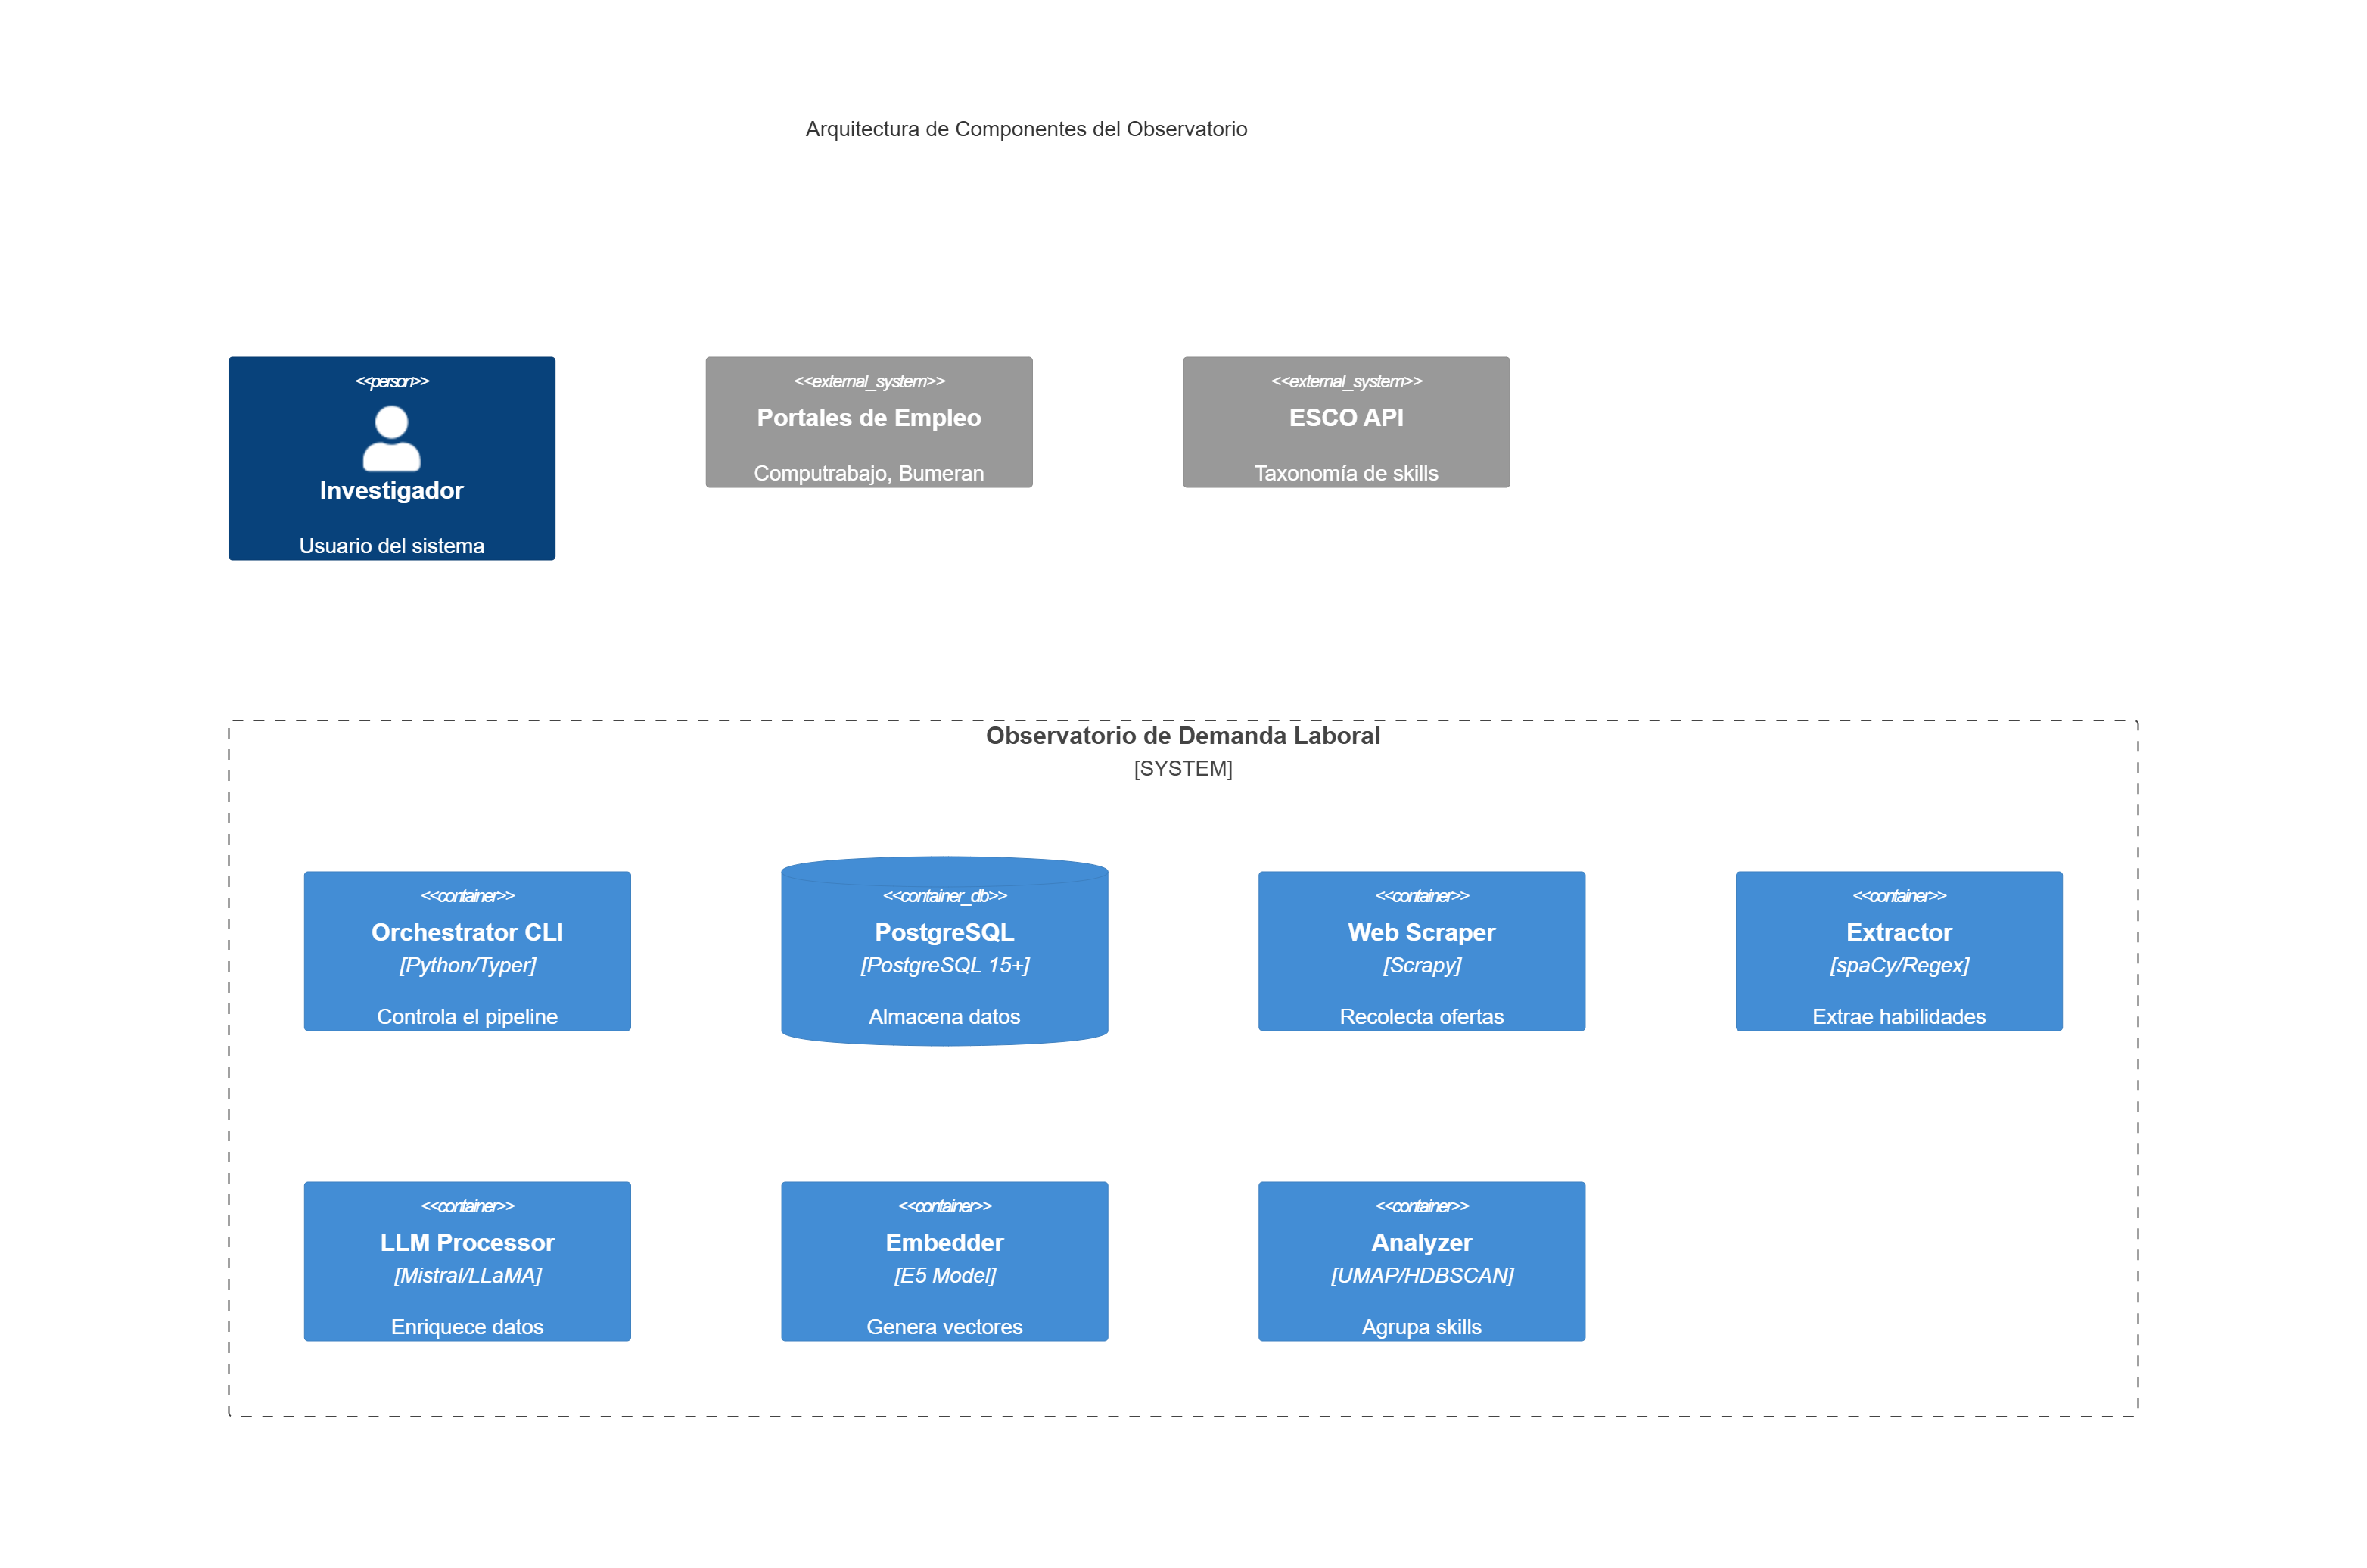
\includegraphics[width=0.95\textwidth]{diagrams/Contexto(Faltan conexiones).png}
\caption{Diagrama de Contexto del Observatorio de Demanda Laboral}
\label{fig:contexto-sistema}
\end{figure}

El sistema interactúa con tres entidades externas principales:

\begin{itemize}
    \item \textbf{Investigador}: Usuario principal del sistema que inicia el proceso de scraping, configura parámetros de análisis y consume los reportes generados.
    \item \textbf{Portales de Empleo}: Fuentes de datos externas (Computrabajo, Bumeran, ElEmpleo) que publican ofertas laborales en formato HTML.
    \item \textbf{ESCO API}: Taxonomía europea de habilidades y competencias utilizada para normalizar y clasificar las habilidades extraídas.
\end{itemize}

Internamente, el sistema está compuesto por siete componentes principales que operan de forma coordinada: Orchestrator CLI (control del pipeline), PostgreSQL (almacenamiento), Web Scraper (adquisición), Extractor (NLP), LLM Processor (enriquecimiento), Embedder (vectorización) y Analyzer (clustering y visualización).

\section{Arquitectura General del Sistema}

\subsection{Pipeline Lineal de 8 Etapas}

El sistema se diseñó como un pipeline secuencial compuesto por ocho módulos especializados que transforman progresivamente los datos brutos en conocimiento estructurado sobre el mercado laboral:

\begin{enumerate}
    \item \textbf{Módulo de Scraping (Scrapy)}: Recolección automatizada de ofertas laborales desde portales web.
    \item \textbf{Módulo de Extracción (NER + Regex)}: Identificación de habilidades explícitas mediante reconocimiento de entidades y patrones.
    \item \textbf{Módulo LLM (Mistral/LLaMA)}: Enriquecimiento semántico y detección de habilidades implícitas.
    \item \textbf{Módulo de Embeddings (E5 Multilingüe)}: Generación de representaciones vectoriales de habilidades.
    \item \textbf{Módulo de Reducción Dimensional (UMAP)}: Proyección a espacios de baja dimensionalidad.
    \item \textbf{Módulo de Clustering (HDBSCAN)}: Agrupamiento no supervisado de habilidades.
    \item \textbf{Módulo de Visualización}: Generación de gráficos y páginas web estáticas.
    \item \textbf{Módulo de Reportes}: Exportación de resultados en formato PDF, PNG y CSV.
\end{enumerate}

\subsection{Representación Visual de la Arquitectura}

La arquitectura del observatorio se presenta desde tres perspectivas complementarias que permiten comprender el sistema en su totalidad: la vista modular detallada, la vista por capas de responsabilidad y la vista de transformación de datos.

\subsubsection{Vista Modular: Pipeline de 8 Etapas}

La Figura \ref{fig:arquitectura-completa} presenta la arquitectura modular completa del sistema, detallando cada una de las ocho etapas del pipeline con sus tecnologías específicas, funciones, entradas, salidas y mecanismos de almacenamiento. Esta vista es fundamental para comprender la responsabilidad individual de cada módulo y cómo estos se integran para formar el sistema completo.

\begin{figure}[H]
\centering
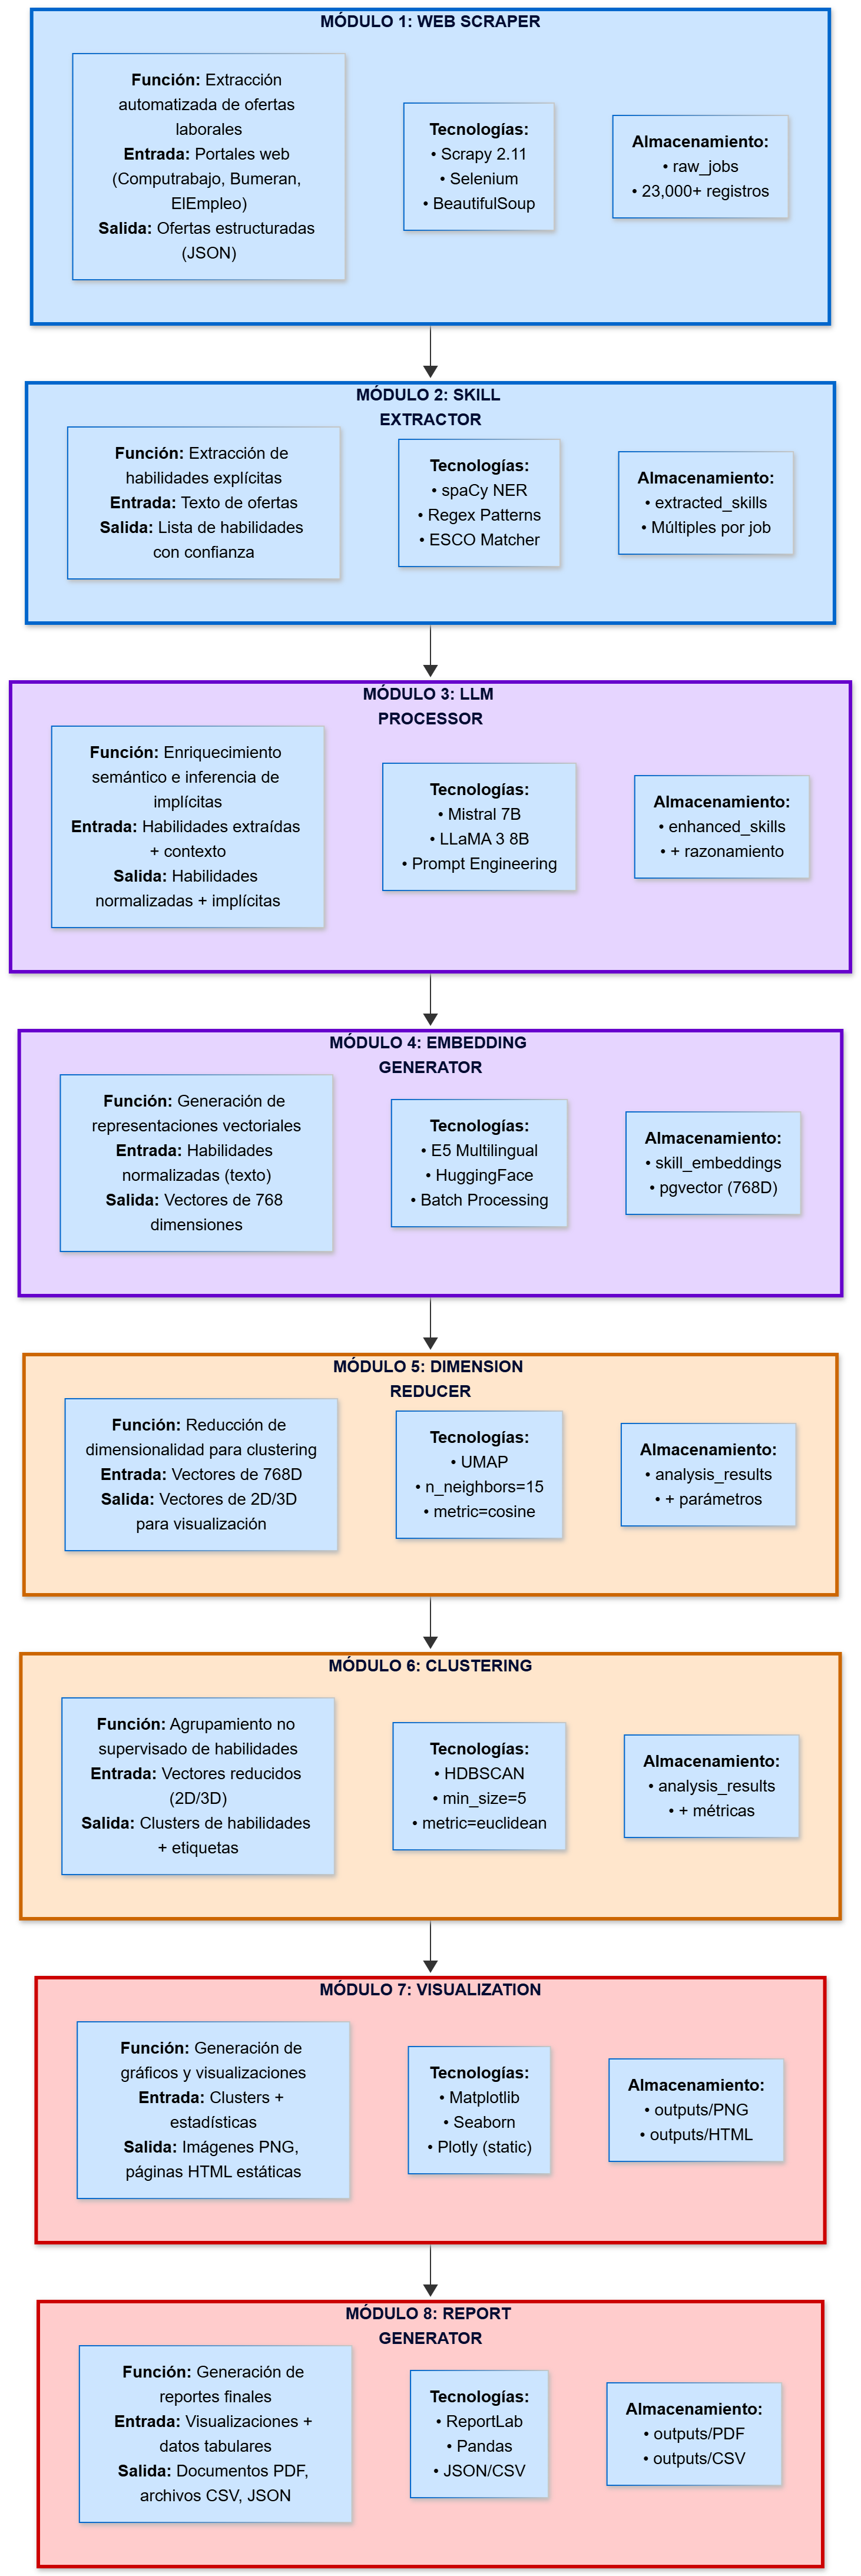
\includegraphics[width=0.45\textwidth]{diagrams/ArquitecturaGeneral.png}
\caption{Arquitectura Modular Completa del Observatorio - Pipeline de 8 Etapas}
\label{fig:arquitectura-completa}
\end{figure}

Cada módulo del pipeline opera de forma autónoma y puede ser ejecutado independientemente, lo que facilita el desarrollo incremental, las pruebas unitarias y la depuración. Los módulos 1-2 se enfocan en la adquisición y extracción inicial de datos; los módulos 3-4 realizan el enriquecimiento semántico mediante inteligencia artificial; los módulos 5-6 ejecutan el análisis no supervisado; y finalmente, los módulos 7-8 generan las salidas consumibles por usuarios finales.

\subsubsection{Vista por Capas: Separación de Responsabilidades}

La Figura \ref{fig:arquitectura-capas} reorganiza los componentes del sistema en siete capas lógicas, mostrando cómo se distribuyen las responsabilidades y cómo fluye el control y los datos entre capas. Esta representación es especialmente útil para comprender la arquitectura desde una perspectiva de ingeniería de software y para identificar las dependencias entre componentes.

\begin{figure}[H]
\centering
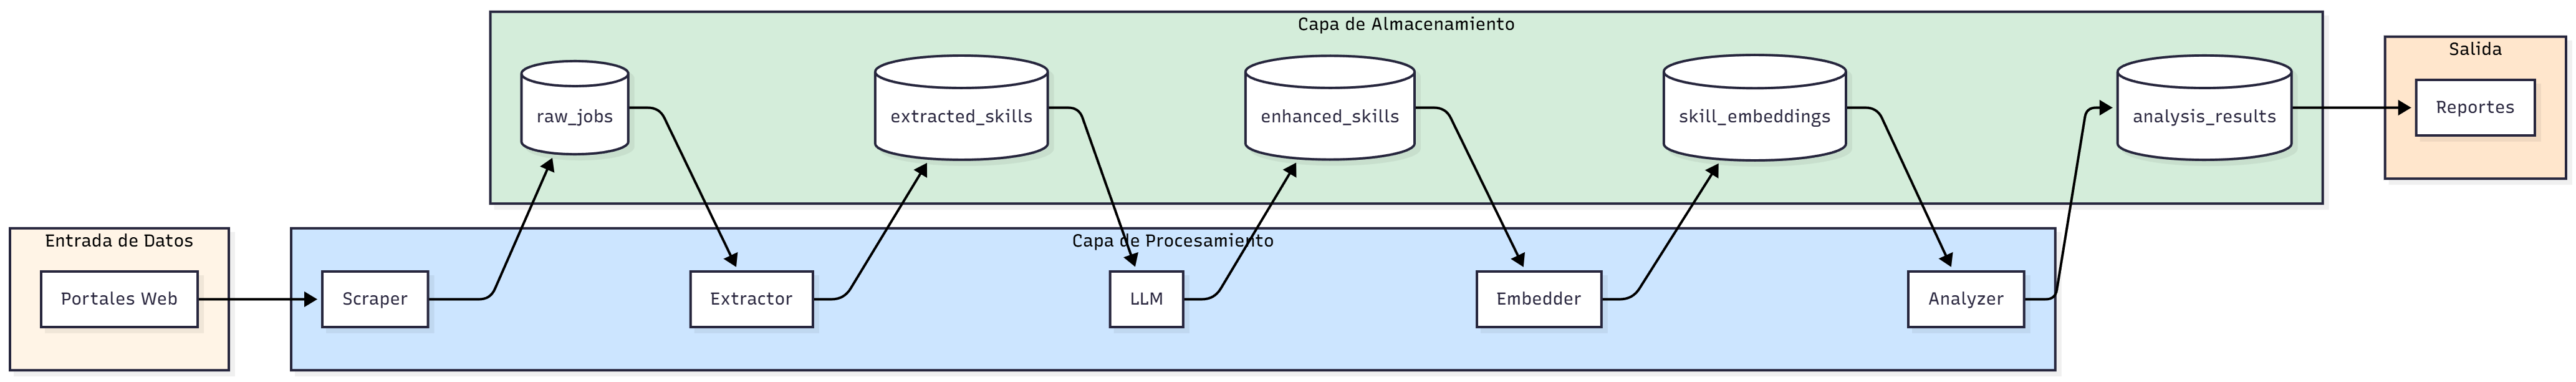
\includegraphics[width=0.95\textwidth]{diagrams/ArquitecturaHorizontal.png}
\caption{Arquitectura en Capas del Sistema - Vista de Separación de Responsabilidades}
\label{fig:arquitectura-capas}
\end{figure}

Las capas 1-5 representan el flujo vertical de procesamiento de datos (de arriba hacia abajo), mientras que la capa 6 (Persistencia) actúa como el repositorio central al que todas las capas superiores acceden para lectura y escritura. La capa 7 (Orquestación) coordina transversalmente la ejecución de todas las demás capas, implementando el patrón de orquestador que controla el ciclo de vida completo del sistema.

\subsubsection{Vista de Estados: Ciclo de Vida de Jobs}

La Figura \ref{fig:estados-jobs} ilustra el ciclo de vida completo que atraviesan las ofertas laborales desde su ingreso al sistema hasta la generación de reportes. Este diagrama de estados muestra las transiciones entre las diferentes etapas de procesamiento, incluyendo los caminos de manejo de errores y reintentos.

\begin{figure}[H]
\centering
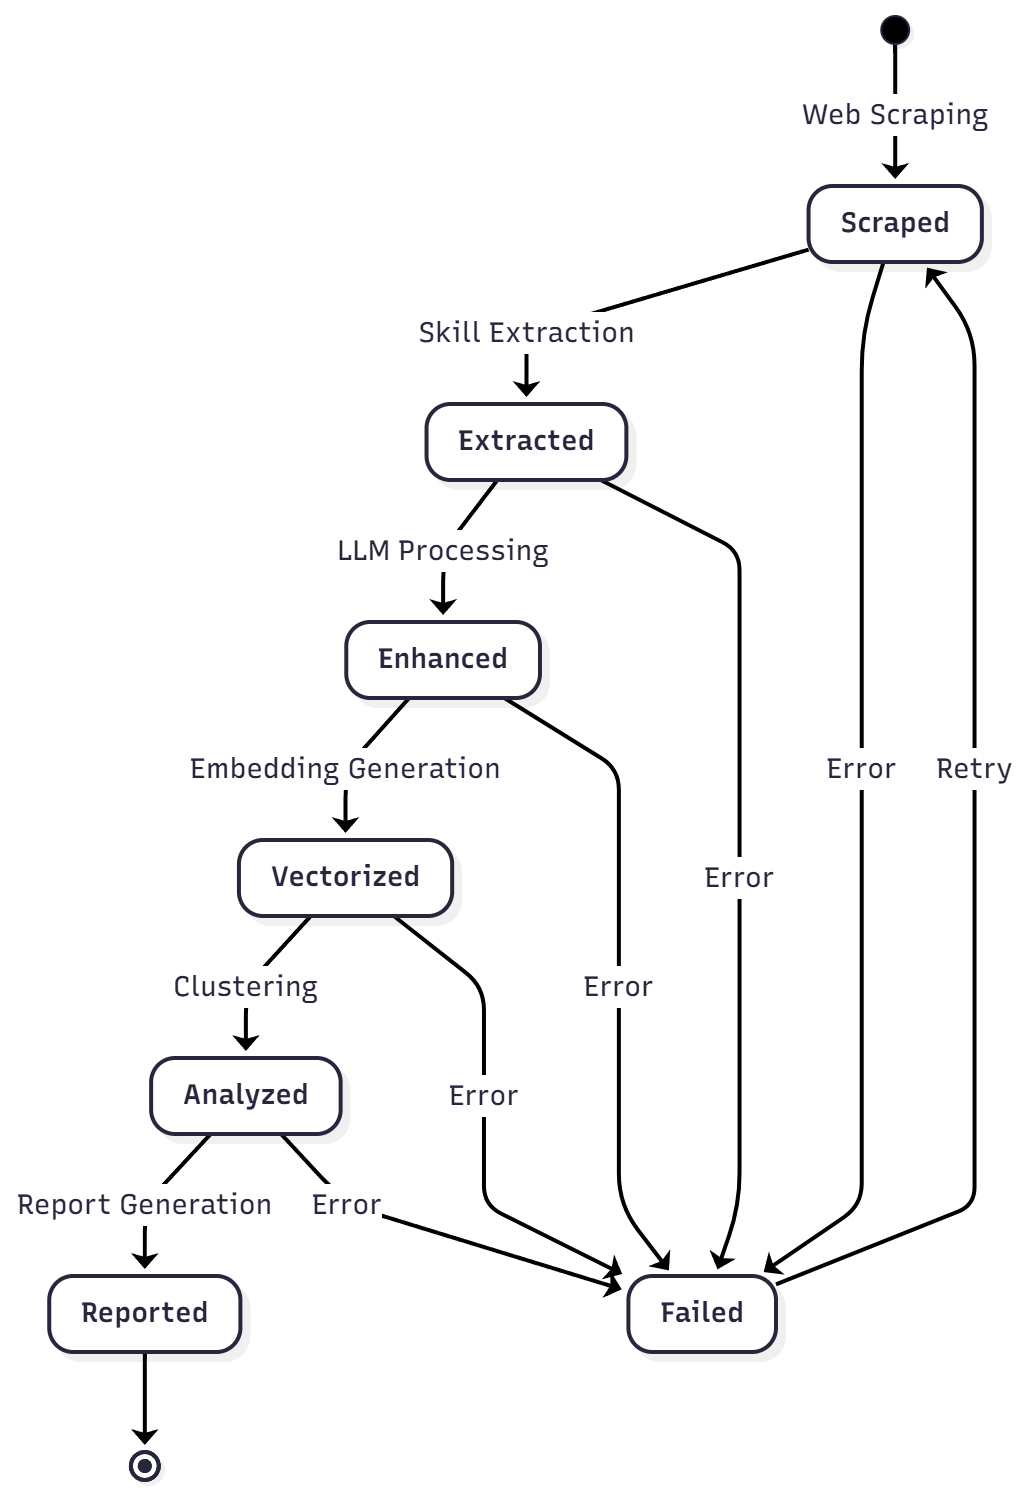
\includegraphics[width=0.6\textwidth]{diagrams/DiagramaEstado.png}
\caption{Diagrama de Estados del Procesamiento de Ofertas Laborales}
\label{fig:estados-jobs}
\end{figure}

Como se observa, los datos atraviesan seis estados principales: \textbf{Scraped} $\rightarrow$ \textbf{Extracted} $\rightarrow$ \textbf{Enhanced} $\rightarrow$ \textbf{Vectorized} $\rightarrow$ \textbf{Analyzed} $\rightarrow$ \textbf{Reported}. En cada transición, el sistema puede detectar errores que llevan al estado \textbf{Failed}, desde donde se pueden aplicar reintentos automáticos. Esta arquitectura de estados garantiza la trazabilidad completa y la capacidad de recuperación ante fallos en cualquier etapa del pipeline.

\section{Diseño de la Base de Datos}

La arquitectura de datos se sustenta en PostgreSQL 15+, seleccionado por su robustez, soporte JSON nativo y capacidad de extensión mediante pgvector para operaciones de similitud vectorial.

\subsection{Esquema de la Base de Datos}

La base de datos está compuesta por seis tablas principales que capturan el flujo completo del pipeline:

\subsubsection{Tabla: raw\_jobs}

Almacena las ofertas laborales tal como fueron extraídas de los portales web:

\begin{verbatim}
CREATE TABLE raw_jobs (
    job_id UUID PRIMARY KEY,
    portal VARCHAR(50) NOT NULL,
    country CHAR(2) NOT NULL,
    url TEXT NOT NULL,
    title TEXT NOT NULL,
    company TEXT,
    location TEXT,
    description TEXT NOT NULL,
    requirements TEXT,
    salary_raw TEXT,
    contract_type VARCHAR(50),
    remote_type VARCHAR(50),
    posted_date DATE,
    scraped_at TIMESTAMP DEFAULT CURRENT_TIMESTAMP,
    content_hash VARCHAR(64) UNIQUE,
    is_processed BOOLEAN DEFAULT FALSE
);
\end{verbatim}

\textbf{Campos clave}:
\begin{itemize}
    \item \texttt{job\_id}: Identificador único generado con UUID v4
    \item \texttt{portal}: Origen de la oferta (computrabajo, bumeran, elempleo)
    \item \texttt{country}: Código ISO 3166-1 alpha-2 (CO, MX, AR)
    \item \texttt{content\_hash}: Hash SHA-256 del contenido para detección de duplicados
    \item \texttt{is\_processed}: Bandera de control para procesamiento incremental
\end{itemize}

\subsubsection{Tabla: extracted\_skills}

Contiene las habilidades identificadas mediante técnicas de NER y expresiones regulares:

\begin{verbatim}
CREATE TABLE extracted_skills (
    extraction_id UUID PRIMARY KEY,
    job_id UUID REFERENCES raw_jobs(job_id),
    skill_text TEXT NOT NULL,
    skill_type VARCHAR(50),
    extraction_method VARCHAR(50),
    confidence_score FLOAT,
    source_section VARCHAR(50),
    span_start INTEGER,
    span_end INTEGER,
    esco_uri TEXT,
    extracted_at TIMESTAMP DEFAULT CURRENT_TIMESTAMP
);
\end{verbatim}

\textbf{Campos clave}:
\begin{itemize}
    \item \texttt{extraction\_method}: Indica el método de extracción (ner, regex, esco\_match)
    \item \texttt{confidence\_score}: Nivel de confianza de la extracción (0-1)
    \item \texttt{source\_section}: Sección de origen (title, description, requirements)
    \item \texttt{span\_start/span\_end}: Posición del span en el texto original
    \item \texttt{esco\_uri}: Enlace a la taxonomía ESCO cuando existe correspondencia
\end{itemize}

\subsubsection{Tabla: enhanced\_skills}

Almacena las habilidades enriquecidas por el procesamiento LLM:

\begin{verbatim}
CREATE TABLE enhanced_skills (
    enhancement_id UUID PRIMARY KEY,
    job_id UUID REFERENCES raw_jobs(job_id),
    original_skill_text TEXT,
    normalized_skill TEXT NOT NULL,
    skill_type VARCHAR(50),
    esco_concept_uri TEXT,
    esco_preferred_label TEXT,
    llm_confidence FLOAT,
    llm_reasoning TEXT,
    is_duplicate BOOLEAN DEFAULT FALSE,
    duplicate_of_id UUID,
    enhanced_at TIMESTAMP DEFAULT CURRENT_TIMESTAMP,
    llm_model VARCHAR(100)
);
\end{verbatim}

\textbf{Campos clave}:
\begin{itemize}
    \item \texttt{normalized\_skill}: Versión normalizada de la habilidad según ESCO
    \item \texttt{skill\_type}: Tipo de habilidad (explicit, implicit, normalized)
    \item \texttt{llm\_confidence}: Confianza del modelo LLM en la inferencia
    \item \texttt{llm\_reasoning}: Justificación del modelo para habilidades implícitas
    \item \texttt{is\_duplicate}: Bandera para habilidades duplicadas identificadas
\end{itemize}

\subsubsection{Tabla: skill\_embeddings}

Contiene las representaciones vectoriales de las habilidades:

\begin{verbatim}
CREATE TABLE skill_embeddings (
    embedding_id UUID PRIMARY KEY,
    skill_text TEXT UNIQUE NOT NULL,
    embedding vector(768) NOT NULL,
    model_name VARCHAR(100) NOT NULL,
    model_version VARCHAR(50),
    created_at TIMESTAMP DEFAULT CURRENT_TIMESTAMP
);

CREATE INDEX ON skill_embeddings
USING ivfflat (embedding vector_cosine_ops)
WITH (lists = 100);
\end{verbatim}

\textbf{Características}:
\begin{itemize}
    \item Utiliza la extensión \texttt{pgvector} para almacenar vectores de 768 dimensiones
    \item Implementa índice IVFFlat para búsquedas de similitud eficientes
    \item Los vectores son generados con el modelo E5 multilingüe
    \item Soporte para operaciones de distancia coseno
\end{itemize}

\subsubsection{Tabla: analysis\_results}

Almacena los resultados de análisis de clustering y tendencias:

\begin{verbatim}
CREATE TABLE analysis_results (
    analysis_id UUID PRIMARY KEY,
    analysis_type VARCHAR(50),
    country CHAR(2),
    date_range_start DATE,
    date_range_end DATE,
    parameters JSONB,
    results JSONB,
    created_at TIMESTAMP DEFAULT CURRENT_TIMESTAMP
);
\end{verbatim}

\textbf{Campos clave}:
\begin{itemize}
    \item \texttt{analysis\_type}: Tipo de análisis (clustering, trends, profile)
    \item \texttt{parameters}: Configuración del análisis en formato JSON
    \item \texttt{results}: Resultados estructurados en formato JSON
    \item Uso de tipo de datos JSONB para flexibilidad y eficiencia en consultas
\end{itemize}

\subsubsection{Tabla: esco\_skills}

Contiene la taxonomía ESCO completa con más de 13,000 habilidades:

\begin{verbatim}
CREATE TABLE esco_skills (
    esco_uri TEXT PRIMARY KEY,
    preferred_label_es TEXT NOT NULL,
    preferred_label_en TEXT,
    alt_labels TEXT[],
    skill_type VARCHAR(50),
    description TEXT,
    skill_reuse_level VARCHAR(50),
    last_updated TIMESTAMP
);
\end{verbatim}

\textbf{Características}:
\begin{itemize}
    \item Integración completa de la taxonomía ESCO v1.1.0
    \item Soporte multilingüe (español e inglés)
    \item Almacenamiento de etiquetas alternativas como array
    \item Metadatos sobre el nivel de reutilización de la habilidad
\end{itemize}

\subsection{Modelo Entidad-Relación}

La Figura \ref{fig:diagrama-er} presenta el modelo entidad-relación completo de la base de datos, mostrando las cinco tablas principales del pipeline y sus relaciones con la tabla de referencia ESCO. Este diagrama ilustra claramente el flujo de datos entre tablas y las dependencias mediante llaves foráneas.

\begin{figure}[H]
\centering
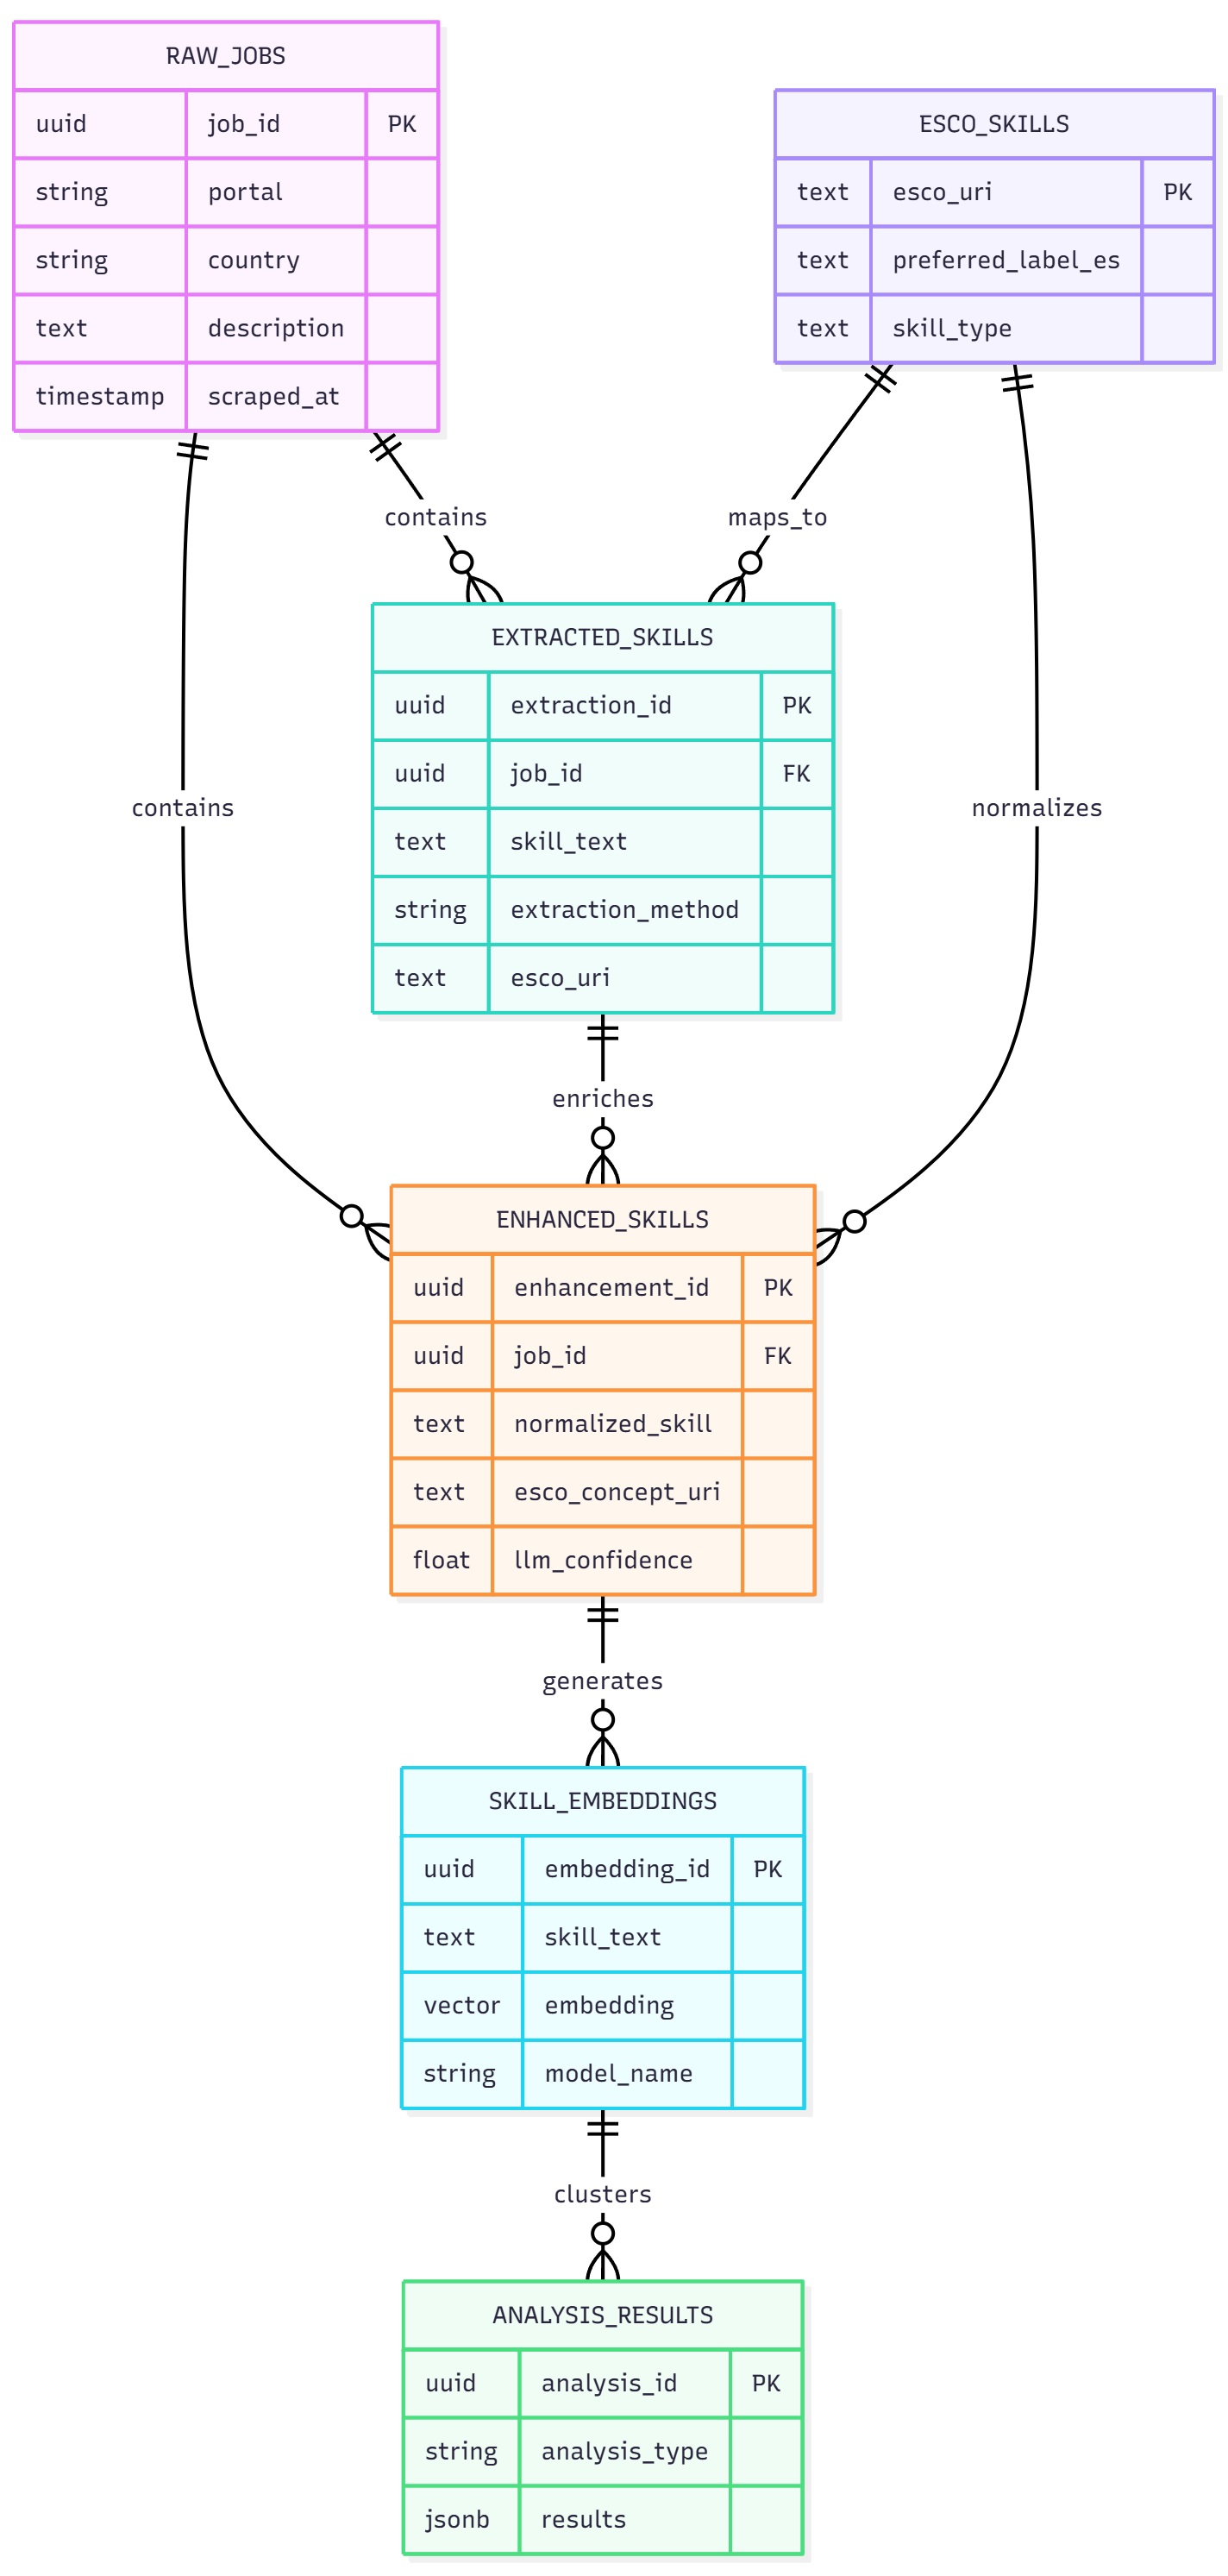
\includegraphics[width=0.5\textwidth]{diagrams/DiagramaER.png}
\caption{Diagrama Entidad-Relación de la Base de Datos del Observatorio}
\label{fig:diagrama-er}
\end{figure}

El modelo de datos sigue una arquitectura de pipeline lineal donde cada tabla representa una etapa de procesamiento:

\begin{itemize}
    \item \texttt{raw\_jobs} es el punto de entrada y contiene referencias (FK) en todas las tablas derivadas
    \item \texttt{extracted\_skills} enriquece (\textit{enriches}) a \texttt{enhanced\_skills}
    \item \texttt{enhanced\_skills} genera (\textit{generates}) vectores en \texttt{skill\_embeddings}
    \item \texttt{skill\_embeddings} alimenta (\textit{clusters}) los resultados en \texttt{analysis\_results}
    \item \texttt{esco\_skills} actúa como tabla de referencia normalizada mediante mapeos desde \texttt{extracted\_skills} y \texttt{enhanced\_skills}
\end{itemize}

Esta arquitectura garantiza integridad referencial y permite trazabilidad completa desde cualquier resultado de análisis hasta la oferta laboral original.

\section{Especificación de Módulos}

\subsection{Módulo 1: Web Scraper}

\textbf{Propósito}: Recolección automatizada de ofertas laborales desde portales de empleo en Colombia, México y Argentina.

\textbf{Tecnologías}:
\begin{itemize}
    \item \textbf{Scrapy 2.11}: Framework asíncrono para scraping a gran escala
    \item \textbf{Selenium + ChromeDriver}: Para portales con contenido dinámico
    \item \textbf{BeautifulSoup 4.12}: Parsing y extracción de HTML
\end{itemize}

\textbf{Características clave}:
\begin{itemize}
    \item Scraping concurrente con límites de tasa por portal
    \item Rotación de user-agents y delays adaptativos
    \item Detección de duplicados mediante hashing de contenido
    \item Reintentos con backoff exponencial ante fallos
    \item Manejo de paginación automática
\end{itemize}

\textbf{Portales soportados}:
\begin{itemize}
    \item Computrabajo (CO, MX, AR)
    \item Bumeran (MX, AR)
    \item ElEmpleo (CO)
    \item InfoJobs (MX)
    \item OCC Mundial (MX)
    \item ZonaJobs (AR)
\end{itemize}

\subsection{Módulo 2: Skill Extractor}

\textbf{Propósito}: Extracción de habilidades explícitas mediante técnicas de NLP.

\textbf{Componentes}:

\begin{enumerate}
    \item \textbf{NER Extractor}: Utiliza spaCy con el modelo \texttt{es\_core\_news\_lg} y un EntityRuler personalizado poblado con la taxonomía ESCO completa para reconocer entidades de tipo skill/technology.

    \item \textbf{Regex Patterns}: Conjunto de expresiones regulares especializadas para capturar tecnologías con nomenclatura específica (ej. ``Node.js'', ``React.js'', ``Python 3.x'').

    \item \textbf{ESCO Matcher}: Módulo de mapeo que normaliza las habilidades extraídas contra la taxonomía ESCO mediante:
    \begin{itemize}
        \item Coincidencia exacta (case-insensitive)
        \item Coincidencia difusa con umbral de similitud
        \item Búsqueda en etiquetas alternativas
    \end{itemize}
\end{enumerate}

\textbf{Pipeline de procesamiento}:
\begin{verbatim}
1. Concatenar: title + description + requirements
2. Preprocesamiento: limpieza y normalización de texto
3. Extracción NER: identificar entidades con EntityRuler
4. Extracción Regex: aplicar patrones de tecnologías
5. Deduplicación: eliminar menciones repetidas
6. Mapeo ESCO: normalizar contra taxonomía
7. Persistencia: almacenar en extracted_skills
\end{verbatim}

\subsection{Módulo 3: LLM Processor}

\textbf{Propósito}: Enriquecimiento semántico de habilidades y detección de competencias implícitas.

\textbf{Modelos soportados}:
\begin{itemize}
    \item \textbf{Mistral 7B Instruct}: Modelo local mediante llama-cpp-python (cuantización Q4)
    \item \textbf{LLaMA 3 8B}: Alternativa con mejor rendimiento en español
    \item \textbf{OpenAI GPT-4}: Fallback opcional mediante API
\end{itemize}

\textbf{Tareas del módulo}:
\begin{enumerate}
    \item \textbf{Deduplicación inteligente}: Identificar variantes de la misma habilidad (``React'', ``React.js'', ``ReactJS'')
    \item \textbf{Inferencia de habilidades implícitas}: Detectar competencias no mencionadas explícitamente pero requeridas por el contexto del cargo
    \item \textbf{Normalización con ESCO}: Mapear todas las habilidades a conceptos ESCO con confianza
    \item \textbf{Razonamiento explicable}: Generar justificaciones para habilidades implícitas
\end{enumerate}

\textbf{Prompt Engineering}: Se diseñaron prompts específicos para el contexto latinoamericano que incluyen:
\begin{itemize}
    \item Instrucciones para manejar ``Spanglish'' (términos técnicos en inglés en contexto español)
    \item Few-shot examples con ofertas laborales reales de la región
    \item Restricción a la taxonomía ESCO para salidas estructuradas
    \item Solicitud de formato JSON con campos definidos
\end{itemize}

\subsection{Módulo 4: Embedding Generator}

\textbf{Propósito}: Generar representaciones vectoriales semánticas de habilidades.

\textbf{Modelo}: \texttt{intfloat/multilingual-e5-base}
\begin{itemize}
    \item Modelo de embeddings multilingüe de 768 dimensiones
    \item Entrenado específicamente para similitud semántica
    \item Soporte nativo para español e inglés en el mismo espacio vectorial
\end{itemize}

\textbf{Proceso}:
\begin{verbatim}
1. Cargar modelo E5 desde Hugging Face
2. Preprocesar: añadir prefijo "query: " según especificación E5
3. Generar embeddings por lotes (batch_size=32)
4. Normalizar vectores (L2 normalization)
5. Almacenar en PostgreSQL con pgvector
6. Crear índice IVFFlat para búsquedas eficientes
\end{verbatim}

\subsection{Módulo 5: Analyzer}

\textbf{Propósito}: Descubrir patrones y clústeres de habilidades mediante análisis no supervisado.

\textbf{Componentes}:

\subsubsection{Reducción de Dimensionalidad (UMAP)}

\textbf{UMAP (Uniform Manifold Approximation and Projection)}:
\begin{itemize}
    \item Reduce los vectores de 768 dimensiones a 2-3 dimensiones
    \item Preserva tanto estructura local como global
    \item Parámetros clave:
    \begin{itemize}
        \item \texttt{n\_neighbors=15}: Balance entre estructura local y global
        \item \texttt{min\_dist=0.1}: Compactación de puntos cercanos
        \item \texttt{metric='cosine'}: Métrica de similitud
    \end{itemize}
\end{itemize}

\subsubsection{Clustering (HDBSCAN)}

\textbf{HDBSCAN (Hierarchical Density-Based Spatial Clustering)}:
\begin{itemize}
    \item Algoritmo de clustering basado en densidad
    \item No requiere especificar número de clústeres
    \item Identifica ruido automáticamente
    \item Parámetros clave:
    \begin{itemize}
        \item \texttt{min\_cluster\_size=5}: Tamaño mínimo de clúster válido
        \item \texttt{min\_samples=3}: Puntos mínimos para densidad
        \item \texttt{metric='euclidean'}: Post-reducción dimensional
    \end{itemize}
\end{itemize}

\subsubsection{Visualización}

Generación de gráficos estáticos:
\begin{itemize}
    \item Scatter plots 2D/3D de clústeres con matplotlib
    \item Distribuciones de frecuencia de habilidades
    \item Heatmaps de co-ocurrencia de habilidades
    \item Gráficos de barras por país y portal
\end{itemize}

\subsubsection{Generación de Reportes}

Exportación multi-formato:
\begin{itemize}
    \item \textbf{PDF}: Reportes completos con ReportLab incluyendo:
    \begin{itemize}
        \item Resumen ejecutivo de hallazgos
        \item Estadísticas descriptivas
        \item Visualizaciones embebidas
        \item Tablas de top skills por clúster
    \end{itemize}
    \item \textbf{PNG}: Imágenes de alta resolución de visualizaciones
    \item \textbf{CSV}: Datos tabulares para análisis externo
    \item \textbf{JSON}: Resultados estructurados para integración
\end{itemize}

\section{Decisiones Técnicas y Justificación}

La siguiente tabla resume las decisiones arquitectónicas clave y su fundamentación:

\begin{longtable}{|p{3.5cm}|p{3.5cm}|p{7cm}|}
\hline
\textbf{Componente} & \textbf{Tecnología} & \textbf{Justificación} \\
\hline
\endfirsthead

\hline
\textbf{Componente} & \textbf{Tecnología} & \textbf{Justificación} \\
\hline
\endhead

\hline
\endfoot

\hline
\endlastfoot

Base de datos & PostgreSQL 15+ & Soporte JSON nativo (JSONB), extensión pgvector para vectores, robustez empresarial, licencia libre (PostgreSQL License). \\
\hline

Taxonomía & ESCO v1.1.0 & Cobertura superior en español (13,000+ skills), etiquetas multilingües, amplia representación de habilidades tecnológicas, respaldo institucional de la Comisión Europea. \\
\hline

Framework de scraping & Scrapy 2.11 & Arquitectura asíncrona para alto rendimiento, manejo robusto de reintentos y errores, middlewares extensibles, amplia comunidad y documentación. \\
\hline

Modelo NLP & spaCy 3.7 + es\_core\_news\_lg & Mejor modelo disponible para español, soporte de EntityRuler para reglas personalizadas, rendimiento optimizado en CPU. \\
\hline

LLM local & Mistral 7B / LLaMA 3 8B & Ejecución local sin dependencia de APIs externas, buen rendimiento en español post-instrucción, cuantización Q4 para reducir requisitos de memoria (4-5 GB RAM). \\
\hline

Modelo de embeddings & intfloat/multilingual-e5-base & Estado del arte en embeddings multilingües, 768 dimensiones balancean expresividad y eficiencia, soporte nativo para español e inglés en espacio compartido. \\
\hline

Algoritmo de clustering & HDBSCAN & No requiere especificar k, identifica ruido, maneja clústeres de densidades variables, jerárquico permite análisis multinivel. \\
\hline

Reducción dimensional & UMAP & Preserva estructura local y global, superior a t-SNE en escalabilidad y reproducibilidad, parámetros interpretables. \\
\hline

Orquestación & Typer CLI & Interface de línea de comandos tipo Git, validación automática de parámetros, ayuda auto-generada, fácil integración con schedulers. \\
\hline

\end{longtable}

\section{Orquestación y Automatización}

\subsection{Flujo de Interacciones entre Componentes}

La Figura \ref{fig:diagrama-secuencia} presenta el diagrama de secuencia que ilustra el flujo completo de interacciones entre los componentes del sistema durante un ciclo de ejecución completo, desde el comando inicial del usuario hasta la generación de reportes finales.

\begin{figure}[H]
\centering
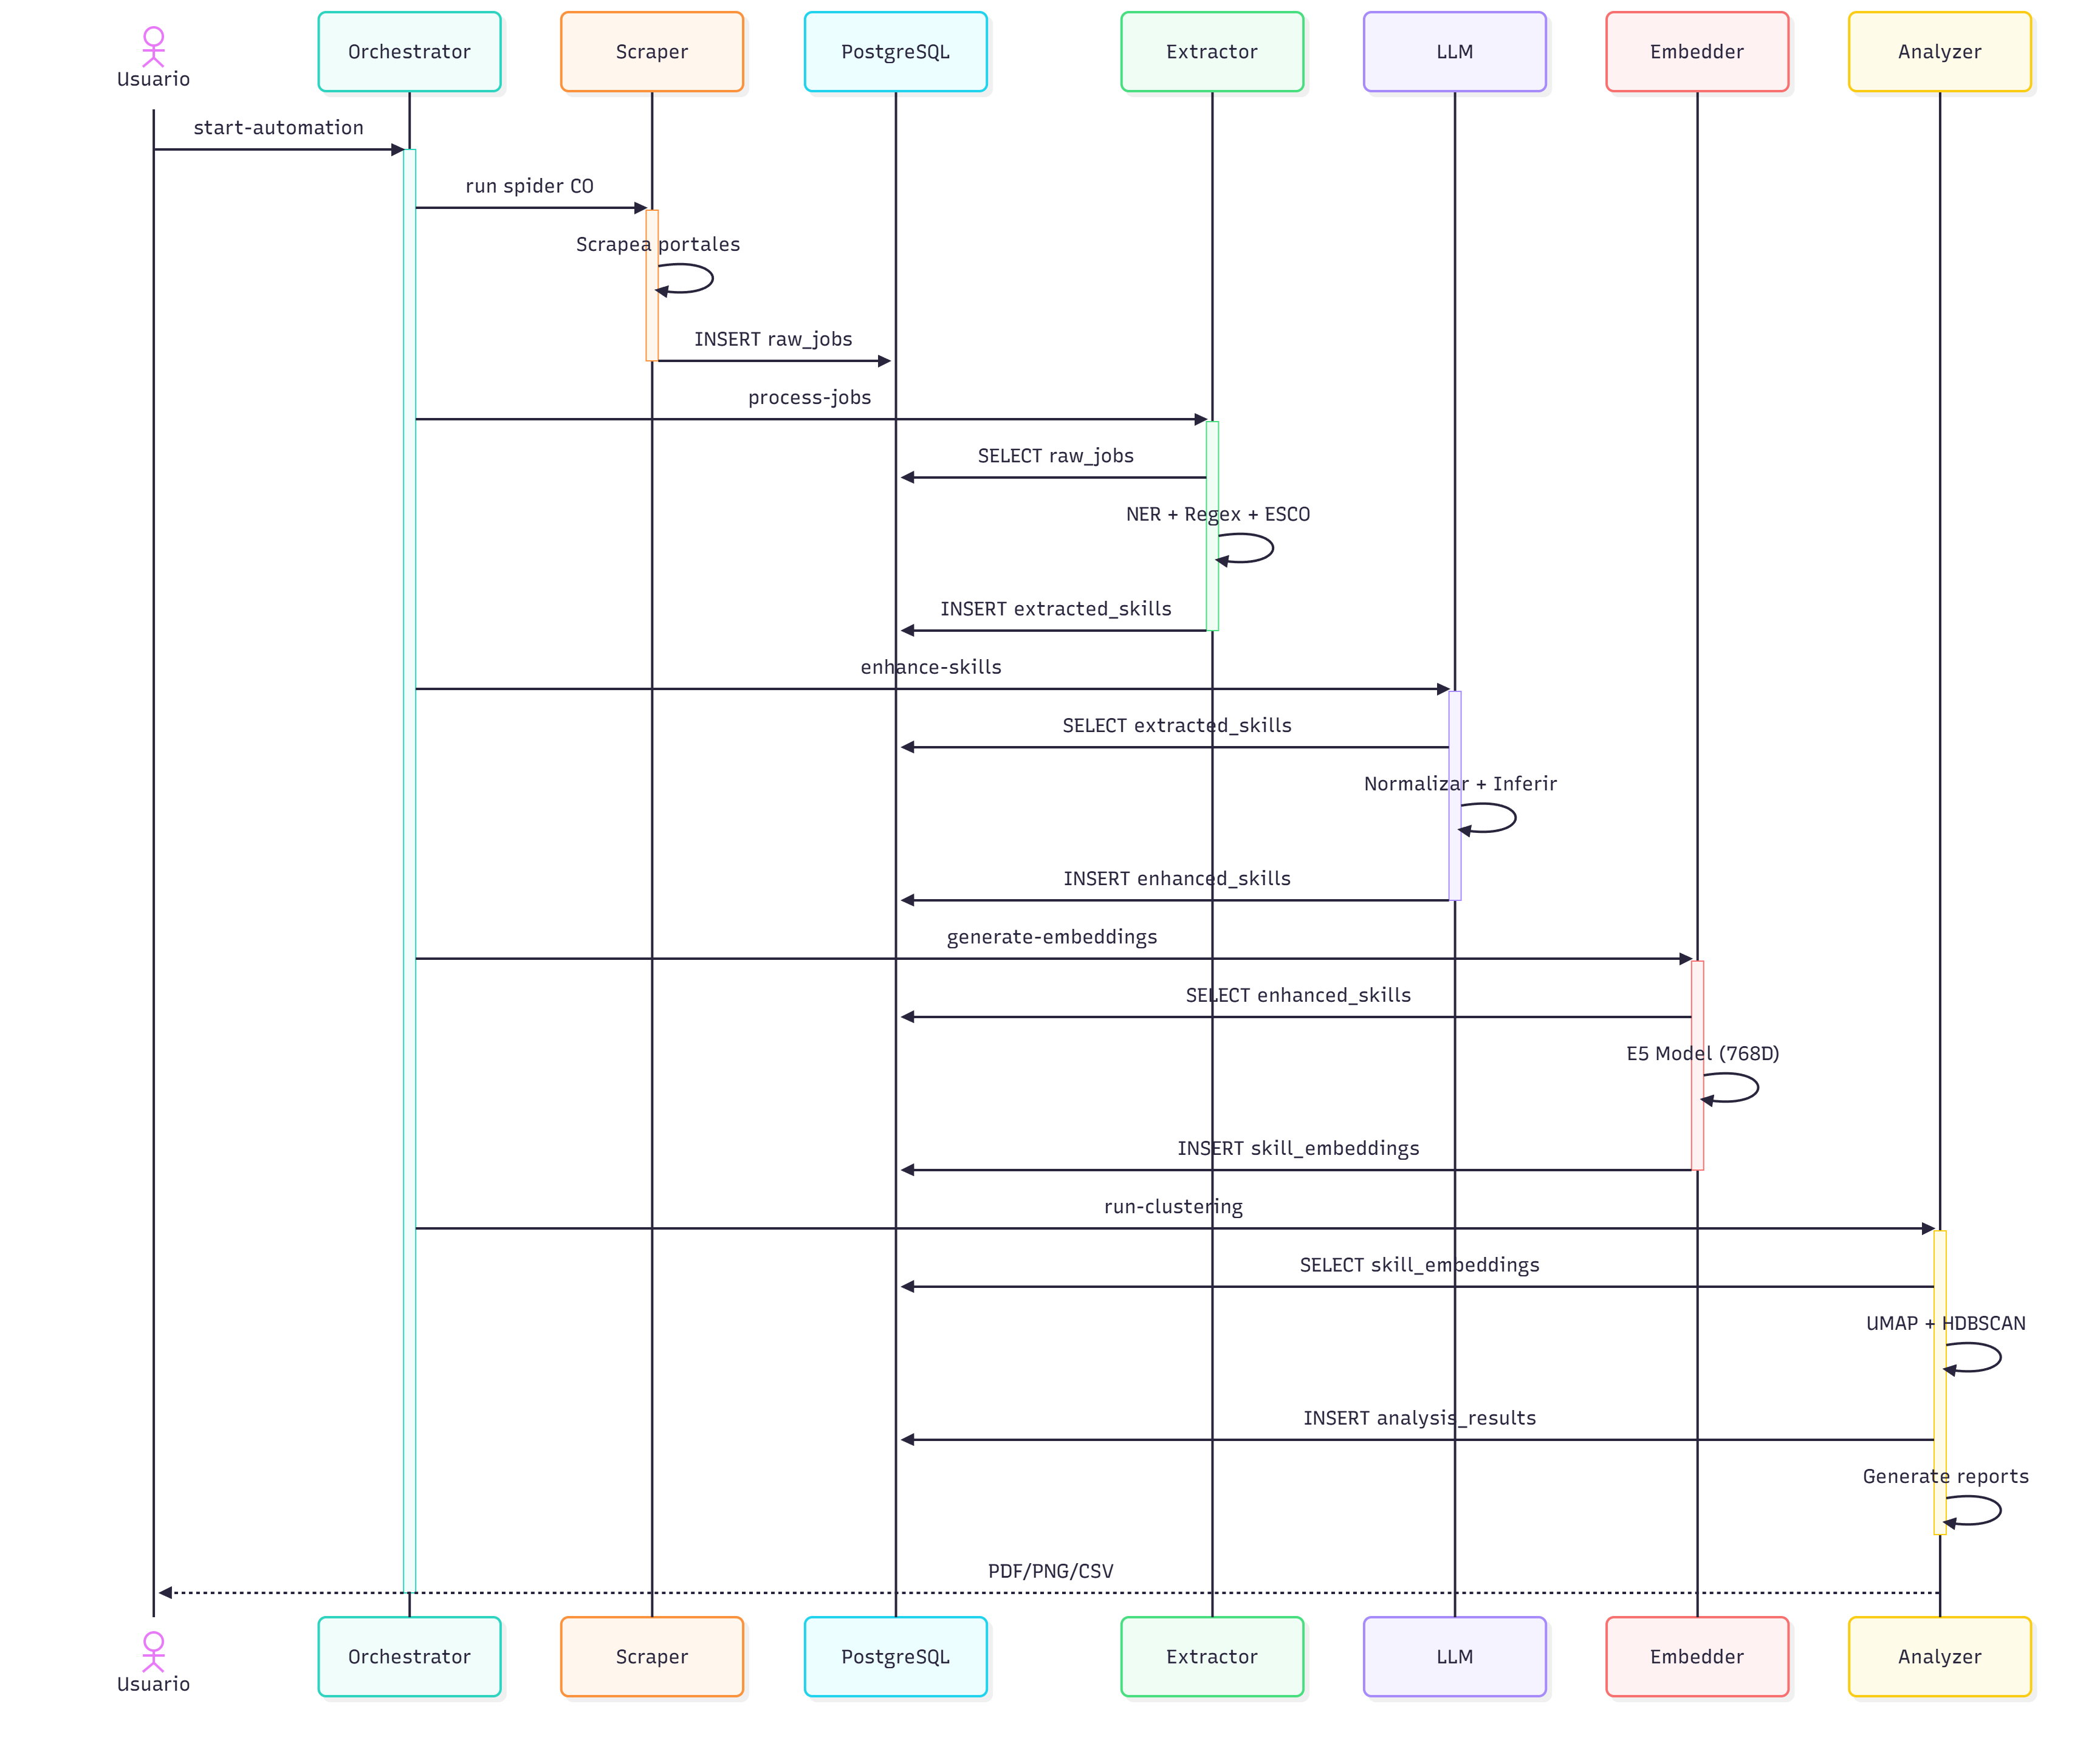
\includegraphics[width=0.95\textwidth]{diagrams/DiagramaSecuencia.png}
\caption{Diagrama de Secuencia de Interacciones del Pipeline Completo}
\label{fig:diagrama-secuencia}
\end{figure}

El flujo de ejecución sigue estos pasos:

\begin{enumerate}
    \item El usuario ejecuta \texttt{start-automation} en el Orchestrator CLI
    \item El Orchestrator lanza el comando \texttt{run spider CO} al módulo Scraper
    \item El Scraper extrae ofertas de los portales web y las inserta en PostgreSQL (\texttt{raw\_jobs})
    \item El Orchestrator ejecuta \texttt{process-jobs}, que activa el Extractor
    \item El Extractor lee ofertas de \texttt{raw\_jobs}, aplica NER + Regex + ESCO, e inserta en \texttt{extracted\_skills}
    \item El Orchestrator ejecuta \texttt{enhance-skills}, que activa el LLM Processor
    \item El LLM lee de \texttt{extracted\_skills}, normaliza e infiere habilidades implícitas, e inserta en \texttt{enhanced\_skills}
    \item El Orchestrator ejecuta \texttt{generate-embeddings}, que activa el Embedder
    \item El Embedder lee de \texttt{enhanced\_skills}, genera vectores 768D con E5 Model, e inserta en \texttt{skill\_embeddings}
    \item El Orchestrator ejecuta \texttt{run-clustering}, que activa el Analyzer
    \item El Analyzer lee de \texttt{skill\_embeddings}, aplica UMAP + HDBSCAN, genera reportes, e inserta resultados en \texttt{analysis\_results}
    \item El Analyzer retorna archivos PDF/PNG/CSV al usuario
\end{enumerate}

Cada paso incluye confirmaciones bidireccionales entre componentes y la base de datos, garantizando consistencia en cada etapa. El manejo de errores permite reintentos en cualquier punto del flujo sin pérdida de datos.

\subsection{Orchestrator CLI}

El sistema se controla mediante un CLI único implementado con Typer:

\begin{verbatim}
python -m src.orchestrator <comando> [opciones]
\end{verbatim}

\textbf{Comandos principales}:
\begin{itemize}
    \item \texttt{run-once <spider> <country>}: Ejecutar scraping único
    \item \texttt{run <spiders> <country>}: Ejecutar múltiples spiders
    \item \texttt{process-jobs}: Procesar ofertas pendientes
    \item \texttt{status}: Estado del sistema y estadísticas
    \item \texttt{health}: Métricas de salud del sistema
    \item \texttt{start-automation}: Iniciar sistema automatizado
    \item \texttt{automation-status}: Estado del scheduler
    \item \texttt{list-jobs}: Listar trabajos programados
\end{itemize}

\subsection{Sistema de Automatización}

Tres componentes coordinan la operación 24/7:

\begin{enumerate}
    \item \textbf{Master Controller}: Coordinador central que gestiona el ciclo de vida del sistema
    \item \textbf{Intelligent Scheduler}: Basado en APScheduler, programa ejecuciones periódicas de spiders con estrategias adaptativas
    \item \textbf{Pipeline Automator}: Detecta nuevos trabajos y los procesa automáticamente a través del pipeline de extracción
\end{enumerate}

\textbf{Programación de spiders}:
\begin{itemize}
    \item Frecuencia configurable por portal (cada 6-12 horas)
    \item Ventanas de ejecución para minimizar detección
    \item Priorización dinámica basada en tasa de actualización del portal
    \item Reintentos automáticos con backoff exponencial
\end{itemize}

\section{Métricas de Evaluación}

\subsection{Métricas por Módulo}

\subsubsection{Scraper}
\begin{itemize}
    \item \textbf{Tasa de éxito}: (peticiones exitosas / peticiones totales) × 100
    \item \textbf{Tasa de parseo}: (trabajos parseados / páginas scrapeadas) × 100
    \item \textbf{Tasa de duplicados}: (trabajos duplicados / trabajos totales) × 100
    \item \textbf{Cobertura}: trabajos únicos por portal por país
\end{itemize}

\subsubsection{Extractor}
\begin{itemize}
    \item \textbf{Precisión}: habilidades validadas / habilidades extraídas
    \item \textbf{Recall}: habilidades extraídas / habilidades anotadas (gold standard)
    \item \textbf{F1-Score}: media armónica de precisión y recall
    \item \textbf{Tasa de mapeo ESCO}: habilidades mapeadas a ESCO / total habilidades
\end{itemize}

\subsubsection{LLM Processor}
\begin{itemize}
    \item \textbf{Tasa de deduplicación}: habilidades deduplicadas / habilidades de entrada
    \item \textbf{Descubrimiento de habilidades implícitas}: habilidades implícitas / total habilidades enriquecidas
    \item \textbf{Éxito de normalización}: habilidades normalizadas con ESCO / total habilidades
    \item \textbf{Tiempo de procesamiento}: tiempo promedio por oferta laboral
\end{itemize}

\subsubsection{Clustering}
\begin{itemize}
    \item \textbf{Silhouette Score}: Medida de cohesión y separación de clústeres (-1 a 1, óptimo $>$ 0.5)
    \item \textbf{Davies-Bouldin Index}: Validez de clústeres (menor es mejor)
    \item \textbf{Estabilidad de clústeres}: Consistencia entre ejecuciones con semillas diferentes
    \item \textbf{Cobertura}: trabajos en clústeres / trabajos totales
\end{itemize}

\subsection{Métricas del Sistema}

\textbf{Métricas de rendimiento}:
\begin{itemize}
    \item Trabajos procesados por hora
    \item Tiempo promedio de extracción por trabajo
    \item Tiempo promedio de procesamiento LLM por trabajo
    \item Tiempo promedio de generación de embedding por habilidad
    \item Latencia de búsqueda de similitud vectorial
\end{itemize}

\textbf{Métricas de calidad}:
\begin{itemize}
    \item F1 Score de extracción de habilidades
    \item Cobertura de enriquecimiento LLM
    \item Silhouette Score de clustering
    \item Tasa de mapeo a ESCO
    \item Consistencia inter-anotadores (para subset validado)
\end{itemize}

\textbf{Objetivo de escala}: El sistema fue diseñado para procesar 600,000 ofertas laborales para la fecha de defensa, con capacidad de crecimiento horizontal mediante:
\begin{itemize}
    \item Particionamiento de tablas por país y fecha
    \item Procesamiento por lotes configurable
    \item Índices optimizados para consultas frecuentes
    \item Caché de embeddings para habilidades recurrentes
\end{itemize}

\chapter{SOLUTION DEVELOPMENT}

This chapter must describe the process utilized to create the solution and relate it to the methodology that was specified in the proposal. Additionally, this chapter must also show the final product. For instance, showing screenshots and describing their functions.

\chapter{RESULTS}

Must present the results of the quality control process, according to what was defined in the methodology. For instance, in a software development project, this section should include the results from standard software testing (unit, functional, system, acceptance, etc.). It is important for them to be consistent with the objective of the project and the methodology used for its development.

This chapter must include an analysis of the results obtained, and conclusions from this analysis.

\chapter{CONCLUSIONS}

\section{Impact Analysis of the Project}

Explain the impact of the results of this project in the short, medium, and long term. It should explain the impact in all of the relevant stakeholders.

\subsection{Impact analysis in systems engineering}

\subsection{Impact analysis in global, economic, environmental, and societal contexts}

\section{Conclusions and Future Work}

Explain whether the goals were accomplished and why. Future work that should be explained based on the project results.


% ============================================================================
% REFERENCIAS
% ============================================================================
\chapter*{REFERENCIAS}
\addcontentsline{toc}{chapter}{REFERENCIAS}
\printbibliography[heading=none]

% ============================================================================
% APÉNDICES
% ============================================================================
\chapter*{APÉNDICES}
\addcontentsline{toc}{chapter}{APÉNDICES}

En esta sección del documento se presenta la lista de todos los apéndices relacionados con el proyecto. Los apéndices deben ser descargables desde el sitio web y deben coincidir con los especificados en la propuesta.

\end{document}
